\section{A constante do círculo} % (fold)
\label{sec:the_circle_constant}

\href{https://tauday.com/tau-manifesto}{\emph{O Manifesto Tau}} é dedicado a um dos números mais importantes da matemática, talvez \emph{o} mais importante: a \emph{constante do círculo}, relacionando a circunferência de um círculo à sua dimensão linear. Por milênios, o círculo foi considerado a mais perfeita das formas, e a constante do círculo captura a geometria do círculo em um número único. Obviamente, a escolha tradicional para a constante da circunferência é $\pi$---mas, como observa o matemático \href{https://www.math.utah.edu/~palais/}{Bob Palais} em seu delicioso artigo ``$\pi$ está errado!'',\footnote{Palais, Robert. ``$\pi$ está errado!'', \emph{The Mathematical Intelligencer}, Volume~23, Number~3, 2001, pp.~7--8. Muitos dos argumentos de \emph{O Manifesto Tau} são baseados ou inspirados por ``$\pi$ está errado!''. O artigo está disponível online em \href{https://www.math.utah.edu/~palais/pi.html}{https://www.math.utah.edu/~palais/pi.html}.} $\pi$ \emph{está errado}. É hora de acertar as coisas.

  \subsection{Uma proposta imodesta} % (fold)
  \label{sec:an_immodest_proposal}

Começamos a reparar os danos causados ​​por $\pi$ compreendendo primeiro o próprio famoso número. A definição tradicional para a constante do círculo estabelece que $\pi$ (pi) é igual à razão entre a circunferência (comprimento) e o diâmetro (largura) de um círculo:\footnote{O símbolo $\equiv$ significa ``é definido como''.}
\begin{equation}
\label{eq:pi}
\pi \equiv \frac{C}{D} = 3,14159265\ldots
\end{equation}
O número $\pi$ tem muitas propriedades notáveis---entre outras coisas, ele é \href{https://pt.wikipedia.org/wiki/N%C3%BAmero_irracional}{\emph{irracional}} e de fato \href{https://pt.wikipedia.org/wiki/N%C3%BAmero_transcendente}{\emph{transcendental}}---e sua presença em fórmulas matemáticas é generalizada.

\begin{figure}
\image{images/figures/circle.pdf}
\caption{Anatomia de um círculo.\label{fig:circle}}
\end{figure}

É óbvio que $\pi$ não está ``errado'' no sentido de estar factualmente incorreto; o número $\pi$ é perfeitamente bem definido e possui todas as propriedades normalmente atribuídas a ele pelos matemáticos. Quando dizemos que ``$\pi$ está errado'', queremos dizer que \emph{$\pi$ é uma escolha confusa e pouco natural para a constante do círculo}. Em particular, um círculo é definido como o conjunto de pontos a uma distância fixa, o \emph{raio}, de um determinado ponto, o \emph{centro} (Figure~\ref{fig:circle}). Embora existam infinitas formas com largura constante (Figure~\ref{fig:constant_width}),\footnote{Imagem obtida de \href{https://commons.wikimedia.org/wiki/File:Reuleaux_triangle_roll.gif}{Wikimedia} em 2019-03-12. Copyright © 2016 de Ruleroll e utilizado sem alteração sob os termos da licença \href{https://creativecommons.org/licenses/by-sa/4.0/deed.pt_BR}{Atribuição-CompartilhaIgual 4.0 Internacional}.} existe apenas uma forma com raio constante. Isso sugere que uma definição mais natural para a constante do círculo poderia usar $r$ no lugar de~$D$:
of~$D$:
\begin{equation}
\label{eq:circle_constant}
\mbox{constante do círculo} \equiv \frac{C}{r}.
\end{equation}
Como o diâmetro de um círculo é o dobro do raio, esse número é numericamente igual a $2\pi$. Como $\pi$, ele é transcendental e, portanto, irracional, e (como veremos na Seção~\ref{sec:the_number_tau}), seu uso na matemática é igualmente difundido.

\begin{figure}
\image{images/figures/Reuleaux_triangle_roll.pdf}
\caption{Uma das infinitas formas não circulares com largura constante.\label{fig:constant_width}}
\end{figure}

Em ``$\pi$ está errado!'', Bob Palais argumenta de forma persuasiva a favor da segunda dessas duas definições para a constante do círculo, e, na minha opinião, ele merece o crédito principal por identificar esse problema e levá-lo a uma ampla audiência. Ele chama a verdadeira constante do círculo de ``uma volta'' e também introduz um novo símbolo para representá-lo (Figura~\ref{fig:palais_tau}). Como veremos, a descrição é presciente, mas infelizmente o símbolo é bastante estranho e (como discutido na Seção~\ref{sec:conflict_and_resistance}), parece improvável que obtenha ampla adoção. (\emph{Atualização}: Isso provou ser realmente o caso, e o próprio Palais se tornou um forte defensor dos argumentos deste manifesto.)

\begin{figure}
\imagebox{images/figures/palais-tau.png}
\caption{O estranho símbolo para a constante do círculo em ``$\pi$ está errado!''.\label{fig:palais_tau}}
\end{figure}

\emph{O Manifesto Tau} é dedicado à proposição de que a melhor resposta a ``$\pi$ está errado'' é ``Não, \emph{é sério}". E a verdadeira constante do círculo merece um nome adequado. Como você já deve ter adivinhado, \emph{O Manifesto Tau} propõe que esse nome seja a letra grega $\tau$ (tau):

\begin{equation}
\label{eq:tau}
\tau \equiv \frac{C}{r} = 6.283185307179586\ldots
\end{equation}
No resto deste manifesto, veremos que o \emph{número} $\tau$ é a escolha correta e mostraremos através do uso (Seção~\ref{sec:the_number_tau} e Seção~\ref{sec:circular_area?) e por argumentação direta (Seção~\ref{sec:conflict_and_resistance}) que a letra $\tau$ também é uma escolha natural.

\subsection{Um inimigo poderoso} % (fold)
 \label{sec:a_powerful_enemy}

Antes de prosseguir com a demonstração de que $\tau$ é a escolha natural para a constante do círculo, vamos primeiro entender o que estamos enfrentando---porque há uma conspiração poderosa, com séculos de idade, determinada a propagar propaganda pró-$\pi$. \href{https://www.amazon.com/exec/obidos/ISBN=0802713327/parallaxproductiA/}{Livros} inteiros \href{https://www.amazon.com/Pi-Sky-Counting-Thinking-Being/dp/0198539568}{são} \href{https://www.amazon.com/exec/obidos/ISBN=0312381859/parallaxproductiA/}{escritos} exaltando as virtudes de $\pi$. (Quero dizer, \href{https://www.amazon.com/exec/obidos/ISBN=0387989463/parallaxproductiA/}{\emph{livros}}!) E devoção irracional a $\pi$ se espalhou até os mais altos níveis da cultura \emph{nerd}; por exemplo, no ``Dia do Pi'' de 2010 o \href{https://www.google.com/}{Google} \emph{mudou seu logo} para homenagear $\pi$ (Figure~\ref{fig:google_pi_day.}).

\begin{figure}
\begin{center}
\image{images/figures/google_pi_day.png}
\end{center}
\caption{O logo do Google em 14 de março (3/14, em notação estadunidense) de 2010 (``Dia do Pi'').\label{fig:google_pi_day.}}
\end{figure}

Enquanto isso, algumas pessoas memorizam dezenas, centenas e até \href{https://www.guinnessworldrecords.com/world-records/most-pi-places-memorised}{\emph{milhares}} de dígitos desse número místico. Que tipo de gente triste memoriza até 40 dígitos de $\pi$ (Figura~\ref{fig:futurama_video})?\footnote{O vídeo na Figurea~\ref{fig:futurama_video} (disponível em \href{https://vimeo.com/12914981}{https://vimeo.com/12914981}) é um trecho de uma palestra proferida pela \href{https://cs.appstate.edu/~sjg/}{Dra.\ Sarah Greenwald}, professora de matemática na \href{https://www.appstate.edu/}{Appalachian State University}. A Dra.\ Greenwald usa referências matemáticas de \emph{Os Simpsons} e \emph{Futurama} para atrair o interesse de seus alunos e ajudá-los a superar sua ansiedade em relação à matemática. Ea também é a mantenedora da Página de Mateática do \href{https://cs.appstate.edu/~sjg/futurama/}{\emph{Futurama}}.}

\begin{figure}
\begin{center}
%= insert_futurama_video
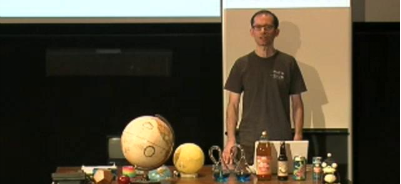
\includegraphics{images/figures/futurama_math_lecture.png} % html_ignore
\end{center}
\caption{\href{https://tauday.com/tau-manifesto/\#sec-about_the_author}{Michael Hartl} prova que \href{https://en.wikipedia.org/wiki/Matt_Groening}{Matt Groening} está errado ao recitar $\pi$ até 40 casas decimais.\label{fig:futurama_video}}
\end{figure}

Certamente, os proponentes do $\tau$ enfrentam um forte oponente. E, no entanto, temos um poderoso aliado---pois a verdade está do nosso lado.

% section the_most_important_number (end)

\section{O número tau} % (fold)
\label{sec:the_number_tau}

Vimos na Seção~\ref{sec:an_immodest_proposal} que o númeroo $\tau$ também pode ser escrito como $2\pi$. Como observado em ``$\pi$ está errado!'', é, portanto, de grande interesse descobrir que a combinação $2\pi$ ocorre com uma frequência surpreendente em todos os campos da matemática. Por exemplo, considere as integrais espaciais em coordenadas polares:
\[
  \int_0^{2\pi}\int_0^\infty f(r, \theta)\, r\, dr\, d\theta.
\]
O limite superior de integração da variável $\theta$ é sempre $2\pi$. O mesmo fator aparece na definição da \href{https://pt.wikipedia.org/wiki/Distribui%C3%A7%C3%A3o_normal}{Distribuição gaussiana (normal)},
\[
  \frac{1}{\sqrt{2\pi}\sigma}e^{-\frac{(x-\mu)^2}{2\sigma^2}},
\]
e, novamente, na \href{https://mathworld.wolfram.com/FourierTransform.html}{transformada de Fourier},
\[
  f(x) = \int_{-\infty}^\infty F(k)\, e^{2\pi ikx}\,dk
\]
\[
    F(k) = \int_{-\infty}^\infty f(x)\, e^{-2\pi ikx}\,dx.
\]
Ela reaparece, também, na \href{https://pt.wikipedia.org/wiki/F%C3%B3rmula_integral_de_Cauchy}{fórmula integral de Cauchy},
\[
  f(a) = \frac{1}{2\pi i}\oint_\gamma\frac{f(z)}{z-a}\,dz,
\]
nas $n$-ésimas \href{https://pt.wikipedia.org/wiki/Raiz_da_unidade}{raízes da unidade},
\[
  z^n = 1 \Rightarrow z = e^{2\pi i/n},
\]
e nos valores da \href{https://pt.wikipedia.org/wiki/Fun%C3%A7%C3%A3o_zeta_de_Riemann}{função zeta de Riemann} para inteiros positivos pares:\footnote{Aqui $B_n$ é o $n$-ésimo \href{https://pt.wikipedia.org/wiki/N%C3%BAmeros_de_Bernoulli}{número de Bernoulli}.}
\[
\begin{split}
  \zeta(2n) & = \sum_{k=1}^\infty \frac{1}{k^{2n}} \\
            & = \frac{|B_{2n}|}{2(2n)!}\,(2\pi)^{2n},\qquad n = 1, 2, 3, \ldots
\end{split}
\]
Estas fórmulas não são escolhidas a dedo---abra seu livro favorito de física ou matemática e tente você mesmo. Há \href{http://www.harremoes.dk/Peter/Undervis/Turnpage/Turnpage1.html}{muitos outros exemplos} e a conclusão é clara: há algo de especial em~$2\pi$.

Para chegar ao fundo deste mistério, devemos retornar aos princípios fundamentais, considerando a natureza dos círculos e, especialmente, a natureza dos \emph{ângulos}. Embora seja provável que grande parte deste material soe familiar, vale a pena revisitá-lo, pois é nesse ponto que o verdadeiro entendimento de $\tau$ começa.

  \subsection{Círculos e ângulos} % (fold)
  \label{sec:circles_and_angles}

Existe uma relação íntima entre círculos e ângulos, como mostra a Figura~\ref{fig:angle_arclength}. Como os círculos concêntricos na Figura~\ref{fig:angle_arclength} têm raios diferentes, as linhas na figura cortam diferentes comprimentos de arco, mas o ângulo~$\theta$ (teta) é o mesmo em cada caso. Em outras palavras, o tamanho do ângulo não depende do raio do círculo usado para definir o arco. A principal tarefa da medição de ângulos é criar um sistema que capte essa invariância com respeito ao raio.

\begin{figure}
\begin{center}
\image{images/figures/angle-arclength.pdf}
\end{center}
\caption{Um ângulo $\theta$ com dois círculos concêntricos.\label{fig:angle_arclength}}
\end{figure}

Talvez o sistema de ângulos mais elementar seja o baseado em \emph{graus}, que divide um círculo em 360 partes iguais. Um resultado desse sistema é o conjunto de ângulos especiais (familiares aos estudantes de trigonometria) mostrados na Figura~\ref{fig:degree_angles}.

\begin{figure}
\begin{center}
\image{images/figures/degree-angles.pdf}
\end{center}
\caption{Alguns ângulos especiais, em graus.\label{fig:degree_angles}}
\end{figure}

Um sistema mais fundamental de medida de ângulo envolve uma comparação direta entre o comprimento do arco $s$ e o raio $r$. Embora os comprimentos na Figura~\ref{fig:angle_arclength} sejam diferentes, o comprimento do arco cresce proporcionalmente ao raio, portanto, a proporção entre o comprimento do arco e o raio é a mesma em cada caso:

\[
s\propto r \Rightarrow \frac{s_1}{r_1} = \frac{s_2}{r_2}.
\]
Isso sugere a seguinte definição de \emph{medida de ângulos em radianos}:
\begin{equation}
\label{eq:radians}
\theta \equiv \frac{s}{r}.
\end{equation}
Essa definição tem a propriedade requerida de ser invariante em relação ao raio e, uma vez que tanto $s$ quanto $r$ têm unidades de comprimento, radianos são \href{https://pt.wikipedia.org/wiki/Magnitude_adimensional}{\emph{adimensionais}} por construção. O uso da medida do ângulo em radianos leva a fórmulas sucintas e elegantes em toda a matemática; por exemplo, a fórmula usual para a derivada de $\sin\theta$ é verdadeira somente quando $\theta$ é expresso em radianos:
\[
  \frac{d}{d\theta}\sin\theta = \cos\theta. \qquad\mbox{(apenas em radianos)}
\]
Naturalmente, os ângulos especiais na Figura~\ref{fig:degree_angles} podem ser expressos em radianos e, quando você estudou trigonometria no ensino médio, você provavelmente memorizou os valores especiais mostrados na Figura~\ref{fig:pi_angles}. (Eu chamo esse sistema de medida $\pi$-radianos para enfatizar que eles são escritos em termos de $\pi$.)


\begin{figure}
\begin{center}
\image{images/figures/pi-angles.pdf}
\end{center}
\caption{Alguns ângulos especiais, em $\pi$-radianos.\label{fig:pi_angles}}
\end{figure}

\begin{figure}
\begin{center}
\image{images/figures/angle-fractions.pdf}
\end{center}
\caption{Os ângulos ``especiais'' são frações de um círculo completo.\label{fig:angle_fractions}}
\end{figure}

Agora, um momento de reflexão mostra que os assim chamados ângulos ``especiais'' nada mais são que frações racionais particularmente simples de um círculo completo, como mostra a Figura~\ref{fig:angle_fractions}. Isso sugere que devemos revisitar a Eq.~\eqref{eq:radians}, reescrevendo o comprimento do arco~$s$ em termos da fração~$f$ da circunferência completa~$C$, ou seja, $s = f C$:
\[ \theta = \frac{s}{r} = \frac{fC}{r} =  f\left(\frac{C}{r}\right) \equiv f\tau. \]
Observe como $\tau$ aparece tão naturalmente nessa análise. Se você acredita em $\pi$, receio que o novo diagrama de ângulos especiais (Figura~\ref{fig:tau_angles}) abale sua fé até o âmago.

\begin{figure}
\begin{center}
\image{images/figures/tau-angles.pdf}
\end{center}
\caption{Alguns ângulos especiais, em radianos.\label{fig:tau_angles}}
\end{figure}

Embora existam muitos outros argumentos em favor de $\tau$, a Figura~\ref{fig:tau_angles} deve ser a mais impressionante. Também vemos na Figura~\ref{fig:tau_angles} a genialidade de Bob Palais ao identificar a constante do círculo como ``\href{https://pt.wikipedia.org/wiki/Volta_(geometria)}{uma volta}'': $\tau$ é a medida do ângulo em radianos para uma \emph{volta} de círculo. Além disso, observe que, com $\tau$ não há \emph{nada para memorizar}: um doze avos de volta é $\tau/12$, um oitavo de volta é $\tau/8$ e assim por diante. Usando $\tau$ nos dá o melhor dos dois mundos, combinando clareza conceitual com todos os benefícios concretos dos radianos; o significado abstrato de, digamos, $\tau/12$ é óbvio, mas também é apenas um número:
\[
\begin{split}
\mbox{um doze avos de volta} = \frac{\tau}{12} & \approx \frac{6.283185}{12} \\
                                             & = 0.5235988.
\end{split}
\]
Finalmente, comparando a Figura~\ref{fig:pi_angles} com a Figura~\ref{fig:tau_angles}, vemos de onde vêm esses fatores \fixme{incômodos} de $2\pi$: uma volta de círculo é $1\tau$, mas $2\pi$. Numericamente, são iguais, mas conceitualmente são bastante distintos.

    \subsubsection{As ramificações} % (fold)
    \label{sec:the_ramifications}

    % subsubsection the_ramifications (end)

Esses fatores desnecessários de $2$ decorrentes do uso de $\pi$ são irritantes por si só, mas muito mais séria é a sua tendência a se \emph{cancelar} quando divididos por qualquer número par. Esses resultados absurdos, como a \emph{metade} de $\pi$ para um \emph{quarto} de volta, ocultam a relação subjacente entre a medida do ângulo e a constante do círculo. Aos que dizem que ``não importa'' se usamos $\pi$ ou $\tau$ quando ensinamos trigonometria, peço apenas que vejam a Figura~\ref{fig:pi_angles}, a Figura~\ref{fig:angle_fractions} e a Figura~\ref{fig:tau_angles} através dos olhos de uma criança. Vocês verão que, da perspectiva de um iniciante, \href{https://tauday.com/a-tau-testimonial}{\emph{usar $\pi$ ao invés de $\tau$ é um desastre pedagógico}}.

  \subsection{As funções do círculo} % (fold)
  \label{sec:the_circle_functions}

Embora a medida do ângulo radiano forneça alguns dos argumentos mais convincentes para a verdadeira constante do círculo, vale a pena comparar as virtudes de $\pi$ e $\tau$ em alguns outros contextos também. Começamos considerando as importantes funções elementares $\sin\theta$ e $\cos\theta$. Conhecidas como as ``funções do círculo'', porque fornecem as coordenadas de um ponto no \emph{círculo unitário} (isto é, um círculo com raio~$1$), seno e cosseno são as funções fundamentais da trigonometria (Figura~\ref{fig:circle_functions}).

\begin{figure}
\begin{center}
\image{images/figures/circle-functions.pdf}
\end{center}
\caption{As funções do círculo são coordenadas no círculo unitário.\label{fig:circle_functions}}
\end{figure}

Vamos examinar os gráficos das funções do círculo para entender melhor seu comportamento.\footnote{Estes gráficos foram produzidos com a ajuda do \href{https://www.wolframalpha.com/}{Wolfram|Alpha}.} Você verá na Figura~\ref{fig:sine_with_tau} e na Figura~\ref{fig:cosine_with_tau} que as duas funções são \emph{periódicas} com período $T$. Como mostra a Figura~\ref{fig:sine_with_tau}, a função seno $\sin\theta$ começa em zero, atinge o máximo em um quarto de período, passa pelo zero em meio período, atinge o mínimo em três quartos de período e retorna a zero após um período completo. Enquanto isso, a função cosseno $\cos\theta$ começa no máximo, tem um mínimo em meio período e passa pelo zero em um quarto e em três quartos de período (Figura~\ref{fig:cosine_with_tau}). Para referência, as duas figuras mostram o valor de $\theta$ (em radianos) em cada ponto especial.

\begin{figure}
\begin{center}
\image{images/figures/sine-with-tau.pdf}
\end{center}
\caption{Pontos importantes de $\sin\theta$ em termos do período $T$.\label{fig:sine_with_tau}}
\end{figure}

\begin{figure}
\begin{center}
\image{images/figures/cosine-with-tau.pdf}
\end{center}
\caption{Pontos importantes de $\cos\theta$ em termos do período $T$.\label{fig:cosine_with_tau}}
\end{figure}

Obviamente, como tanto o seno quanto o cosseno passam por um ciclo completo durante uma volta do círculo, temos que $T = \tau$; ou seja, as funções do círculo têm períodos iguais à constante do círculo. Como resultado, os valores ``especiais'' de $\theta$ são absolutamente naturais: um quarto de período é $\tau/4$, meio período é $\tau/2$, etc. De fato, ao criar a Figura~\ref{fig:sine_with_tau}, a certa altura, me peguei pensando sobre o valor numérico de $\theta$ para o zero da função seno. Como o zero ocorre após meio período e como $\tau \approx 6.28$, um cálculo mental rápido levou ao seguinte resultado:
\[
  \theta_\mathrm{zero} = \frac{\tau}{2} \approx 3.14.
\]
É isso mesmo: fiquei surpreso ao descobrir que \emph{eu já havia esquecido que $\tau/2$ às vezes é chamado de ``$\pi$''}. Talvez isso tenha acontecido com você agora. Bem-vindo ao meu mundo.

  % subsection the_circle_functions (end)

% section radian_angle_measure (end)

   \subsection{A identidade de Euler} % (fold)
   \label{sec:euler_s_identity}

Seria negligente da minha parte não abordar neste manifesto a \emph{identidade de Euler}, às vezes chamada de ``a mais bela equação da matemática''. Essa identidade envolve a \emph{exponencial complexa}, que está profundamente conectada tanto às funções do círculo quanto à sua própria geometria.

Dependendo do caminho escolhido, a seguinte equação pode ser provada como um teorema ou tomada como uma definição; de qualquer forma, ela é notável:
\begin{equation}
\label{eq:eulers_formula}
e^{i\theta} = \cos\theta + i\sin\theta. \qquad\mbox{Fórmula de Euler}
\end{equation}
Conhecida como a \emph{fórmula de Euler} (em honra de \href{https://pt.wikipedia.org/wiki/Leonhard_Euler}{Leonhard Euler}), essa equação relaciona uma exponencial com argumento imaginário às funções do círculo seno e cosseno e à unidade imaginária~$i$. Embora justificar a fórmula de Euler esteja além do escopo deste manifesto, sua origem está acima de qualquer suspeita e sua importância é inquestionável.

Avaliando a Eq.~\eqref{eq:eulers_formula} em $\theta = \tau$ obtemos como resultado a \emph{identidade de Euler}:\footnote{Aqui, eu estou definindo implicitamente a identidade de Euler como \emph{a exponencial complexa da constante do círculo}, em vez de defini-la como a exponencial complexa de qualquer número específico. Se escolhermos $\tau$ como constante do círculo, obtemos a identidade mostrada. Como veremos em breve, essa não é a forma tradicional da identidade, que obviamente envolve $\pi$, mas a versão com $\tau$ é a forma \emph{matematicamente} mais significativa da identidade, de modo que eu acredito que merece esse nome.}
\begin{equation}
\label{eq:eulers_identity_tau}
e^{i\tau} = 1. \qquad\mbox{Identidade de Euler (versão $\tau$)}
\end{equation}
Em palavras, a Eq.~\eqref{eq:eulers_identity_tau} faz a seguinte observação fundamental:

\begin{center}
\emph{A exponencial complexa do círculo é a unidade.}
\end{center}

Geometricamente, multiplicar por $e^{i\theta}$ corresponde à rotação de um número complexo por um ângulo $\theta$ no plano complexo, o que sugere uma segunda interpretação da identidade de Euler:

\begin{center}
\emph{Uma rotação de uma volta é 1.}
\end{center}

\noindent Como o número $1$ é a \href{https://pt.wikipedia.org/wiki/Elemento_neutro}{elemento identidade}, o significado geométrico de $e^{i\tau} = 1$ é que rodar um ponto no plano complexo uma volta completa simplesmente o retorna à sua posição original.

Como no caso da medida de ângulos em radianos, vemos quão natural é a associação entre $\tau$ e uma volta de círculo. De fato, a identificação de $\tau$ com ``uma volta'' faz com que a identidade de Euler soe quase como uma tautologia.\footnote{\href{https://xkcd.com/1475/}{Tecnicamente}, todos os teoremas da matemática são tautologias, mas não sejamos tão pedantes.}

    \subsubsection{Não exatamente a equação mais bonita} % (fold)
    \label{sec:not_the_most_beautiful_equation}

Obviamente, a forma tradicional da identidade de Euler é escrita em termos de $\pi$ ao invés de $\tau$. Para derivá-la, começamos avaliando a fórmula de Euler em $\theta = \pi$, que resulta em
\begin{equation}
\label{eq:eulers_identity_pi}
e^{i\pi} = -1. \qquad\mbox{Identidade de Euler (versão $\pi$)}
\end{equation}
Mas esse sinal de menos é tão feio que a Eq.~\eqref{eq:eulers_identity_pi} é quase sempre reorganizada imediatamente, dando lugar à seguinte equação ``bonita'':
\begin{equation}
\label{eq:eulers_pi_rearranged}
e^{i\pi} + 1 = 0. \qquad\mbox{(reorganizada)}
\end{equation}
Nesse ponto, o expositor geralmente faz uma declaração grandiosa sobre como a Eq.~\eqref{eq:eulers_pi_rearranged} relaciona $0$, $1$, $e$, $i$ e $\pi$---às vezes chhamados de os ``cinco números mais importantes da matemática''.

Nesse contexto, é notável quantas pessoas se queixam que a Eq.~\eqref{eq:eulers_identity_tau} relaciona apenas \emph{quatro} daqueles cinco. Bem:
\begin{equation}
\label{eq:euler_tau_zero}
e^{i\tau} = 1 + 0.
\end{equation}
A Eq.~\eqref{eq:euler_tau_zero}, \emph{sem} reorganização, na verdade relaciona os cinco números mais importantes da matemática: $0$, $1$, $e$, $i$ e $\tau$.\footnote{De fato, a Eq.~\eqref{eq:eulers_identity_tau} pode ser escrita como $e^{i\tau} = 1 + 0i$, o que torna a relação entre os cinco números ainda mais explícita.}

      \subsubsection{Identidades eulerianas} % (fold)
      \label{sec:eulerian_identities}

Como você pode adicionar zero em qualquer lugar de qualquer equação, a introdução de $0$ na Eq.~\eqref{eq:euler_tau_zero} é um contraponto um tanto irônico a $e^{i\pi} + 1 = 0$, mas a identidade $e^{i\pi} = -1$ tem algo sério a dizer. Vejamos o que acontece quando a reescrevemos em termos de $\tau$:
\[
e^{i\tau/2} = -1.
\]
Geometricamente, issi diz que uma rotação de meia volta é o mesmo que multiplicar por $-1$. E, de fato, é esse o caso: quando rotacionado $\tau/2$ radianos, o número complexo $z = a + ib$ é mapeado para $-a - ib$, que é de fato apenas $-1\cdot z$.

Escrita em termos de $\tau$, vemos que a forma ``original'' da identidade de Euler (Eq.~\eqref{eq:eulers_identity_pi}) tem um significado geométrico transparente que faz falta quando escrita em termos de $\pi$. (Obviamente, $e^{i\pi} = -1$ pode ser interpretado como uma rotação de $\pi$ radianos, mas a reorganização quase universal para formar $e^{i\pi} + 1 = 0$ mostra como usar $\pi$ desvia a atenção do significado geométrico natural da identidade.) As identidades de quarto de ângulo têm interpretações geométricas similares: avaliando a Eq.~\eqref{eq:eulers_formula} em $\tau/4$ \fixme{dá} $e^{i\tau/4} = i$, que significa que um quarto de volta no plano complexo é o mesmo que multiplicar por~$i$; similarmente, $e^{i\cdot(3\tau/4)} = -i$ significa que três quartos de volta é o mesmo que multiplicar por~$-i$. Um resumo desses resultados, que chamaremos de \emph{identidades eulerianas}, aparece na Tabela~\ref{table:eulerian_identities}.

\begin{table}
\begin{center}
\begin{tabular}{cllr}
Ângulo de rotação & \multicolumn{3}{c}{Identidade euleriana} \\ \hline
$0$ & $e^{i\cdot0}$ & $ = $ & $1$ \smallskip \\
$\tau/4$ & $e^{i\tau/4}$ & $ = $ & $i$ \smallskip \\
$\tau/2$ & $e^{i\tau/2}$ & $ = $ & $-1$ \smallskip \\
$3\tau/4$ & $e^{i\cdot(3\tau/4)}$ & $ = $ & $-i$ \smallskip \\
$\tau$ & $e^{i\tau}$ & $ = $ & $1$
\end{tabular}
\end{center}
\caption{Identidades eulerianas para rotações de meia-volta, quarto de volta e volta completa.\label{table:eulerian_identities}}
\end{table}

Podemos levar essa análise um passo adiante observando que, para qualquer ângulo~$\theta$, $e^{i\theta}$ pode ser interpretado como um ponto localizado no círculo unitário no plano complexo. Como o plano complexo identifica o eixo horizontal com a parte real do número e o eixo vertical com a parte imaginária, a fórmula de Euler nos diz que $e^{i\theta}$ corresponde às coordenadas $(\cos\theta, \sin\theta)$. Substituindo os valores dos ângulos ``especiais'' da Figura~\ref{fig:tau_angles} na Eq.~\eqref{eq:eulers_formula} fornece, então, os pontos mostrados na Tabela~\ref{table:complex_exponentials} e, plotando esses pontos no plano complexo, produz a Figura~\ref{fig:tau_euler_circle}. Uma comparação da Figura~\ref{fig:tau_euler_circle} com a Figura~\ref{fig:tau_angles} imediatamente elimina quaisquer dúvidas sobre qual opção de constante do círculo revela melhor a relação entre a fórmula de Euler e a geometria do círculo.

\begin{table}
\begin{center}
\begin{tabular}{lcc}
Forma polar & Forma Retangular & Coordenadas \\ \hline\hline
$e^{i\theta}$ & $\cos\theta + i\sin\theta$ & $(\cos\theta, \sin\theta)$ \\ \hline
$e^{i\cdot0}$ & $1$ & $(1, 0)$ \smallskip \\
$e^{i\tau/12}$ & $\frac{\sqrt{3}}{2} + \frac{1}{2}i$ & $(\frac{\sqrt{3}}{2}, \frac{1}{2})$ \smallskip \\
$e^{i\tau/8}$ & $\frac{1}{\sqrt{2}} +  \frac{1}{\sqrt{2}}i$ & $(\frac{1}{\sqrt{2}}, \frac{1}{\sqrt{2}})$ \smallskip \\
$e^{i\tau/6}$ & $\frac{1}{2} +\frac{\sqrt{3}}{2} i$ & $(\frac{1}{2}, \frac{\sqrt{3}}{2})$ \smallskip \\
$e^{i\tau/4}$ & $i$ & $(0, 1)$ \smallskip \\
$e^{i\tau/3}$ & $-\frac{1}{2} +\frac{\sqrt{3}}{2} i$ & $(-\frac{1}{2}, \frac{\sqrt{3}}{2})$ \smallskip \\
$e^{i\tau/2}$ & $-1$ & $(-1, 0)$ \smallskip \\
$e^{i\cdot(3\tau/4)}$ & $-i$ & $(0, -1)$ \smallskip \\
$e^{i\tau}$ & $1$ & $(1, 0)$
\end{tabular}
\end{center}
\caption{Exponenciais complexas dos ângulos especiais da Figura~\ref{fig:tau_angles}.\label{table:complex_exponentials}}
\end{table}

\begin{figure}
\begin{center}
\image{images/figures/tau_euler_circle.pdf}
\end{center}
\caption{Exponenciais complexas de alguns ângulos especiais, plotadas no plano complexo.\label{fig:tau_euler_circle}}
\end{figure}

      % subsubsection eulerian_identities (end)

\section{Área circular: o \emph{golpe de misericórdia}} % (fold)
\label{sec:circular_area}

Se você chegou aqui como um crente em $\pi$, você deve agora estar questionando sua fé. $\tau$ é tão natural, seu significado é tão transparente---será que não há um exemplo em que $\pi$ brilha em toda a sua glória radiante? Uma memória se agita---sim, existe uma fórmula---a fórmula para a área circular! Contemple-a:
\[ A = \tfrac{1}{4} \pi D^2. \]
Espere um pouco. A fórmula da área é sempre escrita em termos do \emph{raio}, assim:
\[ A = \pi r^2. \]
Vemos aqui $\pi$, sem adornos, em uma das equações mais importantes da matemática---uma fórmula provada pela primeira vez pelo próprio \href{https://pt.wikipedia.org/wiki/Arquimedes}{Arquimedes}. A ordem foi restaurada! E, no entanto, o nome desta seção parece ameaçador\ldots\ Se esta equação for a coroação gloriosa de $\pi$, como pode ser também o \href{https://pt.wikipedia.org/wiki/Golpe_de_miseric%C3%B3rdia}{\emph{golpe de misericórdia}}?

  \subsection{Formas quadráticas} % (fold)
  \label{sec:quadratic_forms}

Examinemos esse modelo exemplar de $\pi$, $A = \pi r^2$. Percebemos que ele envolve o diâmetro---não, espere, o \emph{raio}---elevado à segunda potência. Isso faz dele uma \emph{forma quadrática} simples. Tais formas surgem em muitos contextos; como um \href{https://thesis.library.caltech.edu/1940/}{físico}, meus exemplos favoritos vêm do currículo básico de física. Vamos considerá-los um de cada vez.

    \subsubsection{Queda em um campo gravitacional uniforme} % (fold)
    \label{sec:falling_in_a_uniform_gravitational_field}

\href{https://pt.wikipedia.org/wiki/Galileu_Galilei} descobriu que a velocidade de um objeto que cai em um campo gravitacional uniforme é proporcional ao tempo de queda:
\[ v \propto t. \]
A constante de proporcionalidade é a aceleração gravitacional~$g$:
\[ v = g t. \]
Como a velocidade é a derivada da posição, podemos calcular a distância da queda por integração:\footnote{\href{https://xkcd.com/1475/}{Tecnicamente}, todas as integrais devem ser \href{https://mathworld.wolfram.com/DefiniteIntegral.html}{definidas} e a variável de integração deve ser diferente do limite superior (como em $\int_0^t gt'\,dt'$, lido como ``a integral de zero a tê de gê tê linha dê tê linha''.) Esses pequenos \href{https://en.wikipedia.org/wiki/Abuse_of_notation}{abusos de notação} são comuns na física e em outros contextos matemáticos menos formais, como estamos considerando aqui.}
\[ y = \int v\,dt = \int_0^t gt\,dt = \textstyle{\frac{1}{2}} gt^2. \]


    \subsubsection{Energia potencial em uma mola linear} % (fold)
    \label{sec:potential_energy_in_a_linear_spring}

\href{https://pt.wikipedia.org/wiki/Robert_Hooke}{Robert Hooke} descobriu que a força externa necessária para esticar uma mola é proporcional à distância esticada:
\[ F \propto x. \]
A constante de proporcionalidade é a constante de mola~$k$:\footnote{Você pode ter visto isso escrito como $F = -kx$. Nesse caso, $F$ refere-se à força exercida pela \emph{mola}. De acordo com a terceira lei de Newton, a força externa discutida acima é a \emph{negativa} da força da mola.}
\[ F = k x. \]
A energia potencial na mola é, então, igual ao trabalho realizado pela força externa:
\[ U = \int F\,dx = \int_0^x kx\,dx = \textstyle{\frac{1}{2}} kx^2. \]

    \subsubsection{Emergia do movimento} % (fold)
    \label{sec:energy_of_motion}

\href{https://pt.wikipedia.org/wiki/Isaac_Newton}{Isaac Newton} descobriu que a força em um objeto é proporcional à sua aceleração:
\[ F \propto a. \]
A constante de proporcionalidade é a massa~$m$:
\[ F = m a. \]
A energia do movimento, ou \emph{energia cinética}, é igual ao trabalho total realizado ao acelerar a massa até a velocidade~$v$:
\[
\begin{split}
K = \int F\,dx = \int ma\,dx & = \int m\frac{dv}{dt}\,dx \\ & = \int m\frac{dx}{dt}\,dv \\ & = \int_0^v mv\,dv \\ & = \textstyle{\frac{1}{2}} mv^2.
\end{split}
\]

  \subsection{Um pressentimento} % (fold)
  \label{sec:a_sense_of_foreboding}

Tendo visto vários exemplos de formas quadráticas simples na física, você pode agora ter uma sensação de pressentimento quando retornarmos à geometria do círculo. Esse sentimento é justificado.

\begin{figure}
\begin{center}
\image{images/figures/circular-area.pdf}
\end{center}
\caption{Dividindo um círculo em anéis.\label{fig:circular_area}}
\end{figure}


Como visto na Figura~\ref{fig:circular_area}, a área de um círculo pode ser calculada dividindo-a em anéis circulares de comprimento $C$ e largura $dr$, onde a área de cada anel é $C\,dr$:
\[ dA = C\,dr. \]
Agora, a circunferência de um círculo é proporcional ao seu raio:
\[ C \propto r. \]
A constante de proporcionalidade é $\tau$:
\[ C = \tau\,r. \]
A área do círculo é, então, a integral sobre todos os anéis:
\[ A = \int dA = \int_0^r C\,dr = \int_0^r \tau\,r\,dr = \textstyle{\frac{1}{2}} \tau\,r^2. \]

Se você ainda era um partidário de $\pi$ no início desta seção, sua cabeça agora explodiu. Pois vemos que, mesmo neste caso, onde $\pi$ supostamente brilha, de fato há um fator de $2$ ausente. Com efeito, a prova original de Arquimedes não mostra que a área de um círculo é $\pi r^2$, mas que é igual à área de um triângulo retângulo com base $C$ e altura $r$. A aplicação da fórmula para a área triangular fornece, então
\[
  A = \textstyle{\frac{1}{2}} bh = \textstyle{\frac{1}{2}}Cr = \textstyle{\frac{1}{2}}\tau\,r^2.
\]
Simplesmente não há como evitar esse fator de um meio (Tabela~\ref{table:quadratic_forms}).

There is simply no avoiding that factor of a half (Table~\ref{table:quadratic_forms}).

\begin{table}
\begin{center}
\begin{tabular}{lcc}
Quantidade & Símbolo & Expressão \\ \hline
Distância de queda & $y$ & $\textstyle{\frac{1}{2}}gt^2$ \smallskip \\
Energia da mola & $U$ & $\textstyle{\frac{1}{2}}kx^2$ \smallskip \\
Energia cinética & $K$ & $\textstyle{\frac{1}{2}}mv^2$ \smallskip \\
Área do círculo & $A$ & $\textstyle{\frac{1}{2}}\tau\,r^2$
\end{tabular}
\end{center}
\caption{Algumas formas quadráticas comuns.\label{table:quadratic_forms}}
\end{table}

    \subsubsection{Quod erat demonstrandum} % (fold)
    \label{sec:quod_erat_demonstrandum}

Neste manifesto nós nos propusemos a mostrar que $\tau$ é a verdadeira constante do círculo. Como a fórmula para a área do círculo era praticamente o último e o melhor argumento que $\pi$ tinha a seu favor, eu irei contra a maioria aqui e direi: \href{https://pt.wikipedia.org/wiki/Quod_erat_demonstrandum}{Q.E.D.}

    % subsubsection quod_erat_demonstrandum (end)

% section circular_area (end)

\section{Conflito e resistência} % (fold)
\label{sec:conflict_and_resistance}

Apesar da demonstração definitiva da superioridade de $\tau$, no entanto, há muitos que se opõem a ela, tanto como notação quanto como número. Nesta seção, abordamos as preocupações daqueles que aceitam o valor, mas não a letra. Em seguida, refutamos alguns dos muitos argumentos reunidos contra $C/r$ em si, incluindo o chamado ``Manifesto Pi'' que defende a primazia de $\pi$. Nesse contexto, discutiremos o assunto bastante avançado do volume de uma hiperesfera (Seção~\ref{sec:volume_of_a_hypersphere}), que melhora e amplia os argumentos da Seção~\ref{sec:circular_area} sobre a área do círculo.

  \subsection{Uma volta} % (fold)
  \label{sec:one_turn}

O verdadeiro teste de qualquer notação é o uso; tendo visto $\tau$ ser usado ao longo deste manifesto, você já deve estar convencido de que ele desempenha bem seu papel. Mas para uma constante tão fundamental quanto $\tau$ seria bom termos algumas razões mais profundas para a nossa escolha. Por que não $\alpha$, por exemplo, ou $\omega$? O que há de tão especial sobre o $\tau$?

Há duas razões principais para usar $\tau$ para a constante do círculo. A primeira é que $\tau$ se assemelha visualmente a $\pi$: após séculos de uso, a associação de $\pi$ com a constante do círculo é inevitável, e usar $\tau$ se alimenta dessa associação em vez de combatê-la. (De fato, a linha horizontal em cada letra sugere que interpretemos as ``pernas'' como \emph{denominadores}, de modo que $\pi$ tem duas pernas em seu denominador, enquanto $\tau$ tem apenas uma. Visto dessa maneira, a relação $\tau = 2\pi$ é perfeitamente natural.)\footnote{Agradeço a Jim Porter, leitor de \emph{O Manifesto Tau}, por apontar esta interpretação.}

A segunda razão é que $\tau$ corresponde a uma \emph{volta} ou um \emph{turno} de círculo e você deve ter percebido que tanto ``$\tau$'' quanto ``turno'' começam com um som ``\emph{t}''. Essa foi a motivação original para a escolha de $\tau$ e não é uma coincidência: a raiz da palavra ``turno'' é a palavra grega τόρνος (tornos), que significa ``torno''. Usar uma fonte matemática para a primeira letra em τόρνος nos dá: $\tau$.

Depois do lançamento original de \emph{O Manifesto Tau}, eu descobri que \href{http://www.harremoes.dk/Peter/}{Peter Harremo\"{e}s} propôs independentemente o uso de $\tau$ para o autor de ``$\pi$ Está Errado!'', Bob Palais, em 2010, que John Fisher propôs $\tau$ em um \href{https://groups.google.com/forum/#!msg/sci.math/c-DHmJHSA0A/sLCoOtHB1UAJ}{post da Usenet} em 2004 e que Joseph Lindenberg antecipou tanto o argumento quanto o símbolo mais de vinte anos antes!\footnote{Lindenberg incluiu o seu manuscrito datilografado original e muitos outros argumentos em seu site \href{https://sites.google.com/site/taubeforeitwascool/}{\emph{Tau Before It Was Cool}}.} O Dr.~Harremo\"{e}s, em particular, enfatizou a importância de uma observação feita na Seção~\ref{sec:an_immodest_proposal}: usar $\tau$ dá à contante do círculo um \emph{nome}. Como $\tau$ é uma letra grega comum, as pessoas que a encontram pela primeira vez podem pronunciá-la imediatamente. Além disso, diferentemente de chamar a constante do círculo de uma ``volta'', $\tau$ funciona bem em contextos escritos e falados. Por exemplo, dizer que um quarto de círculo tem a medida do ângulo em radianos ``um quarto de volta'' parece ótimo, mas ``virar quatro radianos'' soa estranho e ``a área de um círculo é meia volta $r$ ao quadrado'' soa absolutamente bizarro. Usando $\tau$, podemos dizer ``tau sobre quatro radianos'' e ``a área de um círculo é meio tau $r$ ao quadrado''.

    \subsubsection{Notação Ambígua} % (fold)
    \label{sec:ambiguous_notation}


Obviamente, com qualquer nova notação, existe o potencial de conflito com o uso corrente. Conforme observado na Seção~\ref{sec:an_immodest_proposal}, ``$\pi$ Está Errado!'' evita esse problema introduzindo um novo símbolo (Figura~\ref{fig:palais_tau}). Há precedentes para isso; por exemplo, nos primórdios da mecânica quântica, \href{https://pt.wikipedia.org/wiki/Max_Planck}{Max Planck} introduziu a constante~$h$, que relaciona a energia de uma partícula de luz à sua frequência (através de $E = h\nu$), mas os físicos logo perceberam que é frequentemente mais conveniente usar $\hbar$ (leia ``h-barra'')---onde $\hbar$ é apenas $h$ dividido por\ldots\ hum\ldots\ $2\pi$---e esse uso agora é padrão.

Porém, fazer um novo símbolo ser aceito é difícil: ele precisa de um nome, esse nome deve ser popularizado e o próprio símbolo deve ser adicionado aos sistemas de processamento de texto e de tipografia. Além disso, promulgar um novo símbolo para $2\pi$ exigiria a cooperação da comunidade acadêmica matemática, a qual em matéria de $\pi$ vs. $\tau$ tem sido, até agora, apática na melhor das hipóteses e hostil na pior. Usar um símbolo existente ajuda a vencer essa resistência.\footnote{Talvez algum dia os matemáticos acadêmicos cheguem a um consenso sobre um símbolo diferente para o número $2\pi$; se isso acontecer, reservo-me o direito de apoiar a notação que propuserem. Mas eles já tiveram mais de 300 anos para consertar esse problema do $\pi$, de modo que eu pretendo esperar sentado.}

Em vez de advogar um novo símbolo, \emph{O Manifesto Tau} opta pelo uso de uma letra grega existente. Como resultado, como $\tau$ já é usado em alguns contextos atuais, precisamos resolver os conflitos com a prática existente. Felizmente, há surpreendentemente poucos usos comuns. Além disso, enquanto $\tau$ é usado para determinadas variáveis \emph{específicas}---por exemplo, \emph{tensão de cisalhamento} na engenharia mecânica, \emph{torque} na mecânica rotacional e \emph{tempo próprio} na relatividade especial e na geral---não há uso conflitante \emph{universal}.\footnote{A única exceção possível a isso é a \emph{proporção áurea}, que é frequentemente denotada por $\tau$ na Europa. Mas não há apenas uma alternativa comum para essa notação---a letra grega $\varphi$---este uso mostra que há precedentes para o uso de $\tau$ para denotar uma constante matemática fundamental.} Nesses casos, podemos tolerar a ambiguidade ou contornar os poucos conflitos presentes, alterando seletivamente a notação, como usar $N$ para o torque\footnote{Essa alternativa para o torque já está em uso; veja, por exemplo, \emph{Introduction to Electrodynamics}, de David Griffiths, p.~162.} ou $\tau_p$ para o tempo próprio.

Apesar desses argumentos, potenciais conflitos de uso provaram ser a maior fonte de resistência ao $\tau$. Alguns correspondentes chegaram a negar categoricamente que $\tau$ (ou, presumivelmente, qualquer outro símbolo atualmente em uso) poderia superar esses problemas. Mas cientistas e engenheiros têm uma alta tolerância à ambiguidade notacional e alegar que $\tau$-a-constante-do-círculo não pode coexistir com outros usos ignora consideráveis evidências ​​em contrário.

Um exemplo de ambiguidade facilmente tolerada ocorre na mecânica quântica, onde encontramos a seguinte fórmula para o \emph{raio de Bohr}, que (\emph{grosso modo}) é o ``tamanho'' de um átomo de hidrogênio em seu estado de energia mais baixo (o \emph{estado fundamental}):

\[
a_0 = \frac{\hbar^2}{m e^2},
\]
onde $m$ é a massa de um elétron e $e$ é a sua carga. Enquanto isso, o próprio estado fundamental é descrito por uma quantidade conhecida como \href{https://pt.wikipedia.org/wiki/Fun%C3%A7%C3%A3o_de_onda}{função de onda}, que cai exponencialmente com o raio em uma escala de comprimento definida pelo raio de Bohr:
\begin{equation}
\label{eq:hydrogen}
\psi(r) = N\,e^{-r/a_0},
\end{equation}
onde $N$ é uma constante de normalização.

Já percebeu o problema? Provavelmente não, e esse é exatamente o ponto. O ``problema'' é que o $e$ no raio de Bohr e o $e$ na função de onda \emph{não são os mesmos $e$}---o primeiro é a carga de um elétron, enquanto o segundo é o número natural (a base dos logaritmos naturais). De fato, se expandirmos o fator de $a_0$ no argumento do expoente na Eq.~\eqref{eq:hydrogen}, obtemos
\[
\psi(r) = N\,e^{-m e^2 r/\hbar^2},
\]
que tem um $e$ elevado à potência de algo com $e$ em si. É ainda pior do que parece, porque o próprio $N$ também contém $e$:
\[
\psi(r) = \sqrt{\frac{1}{\pi a_0^3}}\,e^{-r/a_0} =
\frac{m^{3/2} e^3}{\pi^{1/2} \hbar^3}\,e^{-m e^2 r/\hbar^2}.
\]

Não tenho dúvidas de que, se uma notação separada para o número natural ainda não existisse, qualquer um propondo a letra $e$ ouviria que é impossível por causa dos conflitos com outros usos. E, no entanto, na prática, ninguém nunca teve nenhum problema em usar $e$ nos dois contextos acima.
Há muitos outros exemplos, incluindo situações em que até $\pi$ é usado para duas coisas diferentes.\footnote{Veja, por exemplo, \emph{An Introduction to Quantum Field Theory}, de Peskin e Schroeder, onde $\pi$ é usado tanto para denotar a constante do círculo quanto um ``momento conjugado'' na mesma página (p.~282).} É difícil entender em que seria diferente usar $\tau$ para denotar múltiplas quantidades.

A propósito, o $\pi$-pedantes por aí (e provaram ser muitos) podem notar que a função de onda no estado fundamental do hidrogênio tem um fator de $\pi$:
\[
\psi(r) = \sqrt{\frac{1}{\pi a_0^3}}\,e^{-r/a_0}.
\]
À primeira vista, isso parece ser mais natural do que a versão com $\tau$:
\[
\psi(r) = \sqrt{\frac{2}{\tau a_0^3}}\,e^{-r/a_0}.
\]
Como sempre, as aparências enganam: o valor de $N$ vem do produto
\[
\frac{1}{\sqrt{2\pi}} \frac{1}{\sqrt{2}} \frac{2}{a_0^{3/2}},
\]
que mostra que a constante do círculo entra no cálculo através de $1/\sqrt{2\pi}$, ou seja, $1/\sqrt{\tau}$. Tal como acontece com a fórmula da área do círculo, que o cancelamento deixe um $\pi$ \fixme{nu} é uma mera coincidência.

    % subsubsection ambiguous_notation (end)

  \subsection{O Manifesto Pi} % (fold)
  \label{sec:the_pi_manifesto_a_rebuttal}

Embora a maioria das objeções a $\tau$ venham de correspondência dispersa por email e de comentários diversos na Web, há também uma resistência organizada. Em particular, desde a publicação de \emph{O Manifesto Tau}, em junho de 2010, um ``\href{http://www.thepimanifesto.com/}{Manifesto Pi}'' surgiu para argumentar em favor da constante do círculo tradicional. Esta seção e as duas seguintes contêm uma refutação de seus argumentos. Por necessidade, esse tratamento é mais sucinto e mais avançado que o restante do manifesto, mas mesmo uma leitura superficial do que se segue dará uma impressão da fraqueza do argumento do Manifesto Pi.

Embora possamos certamente considerar o surgimento do Manifesto Pi um bom sinal do interesse contínuo nesse assunto, ele faz várias alegações falsas. Por exemplo, ele diz que o fator de $2\pi$ na distribuição gaussiana (normal) é uma coincidência e que ela pode ser escrita mais naturalmente como
\[
\frac{1}{\sqrt\pi(\sqrt 2\sigma)}e^{\frac{-x^2}{(\sqrt 2\sigma)^2}}.
\]
Isso está errado: o fator de $2\pi$ resulta da elevação ao quadrado da distribuição gaussiana não normalizada e da conversão para coordenadas polares, o que leva a um fator de $1$ a partir da integral radial e a $2\pi$ a partir da integral angular. Como no caso da área d círculo, o fator de $\pi$ vem de $1/2\times 2\pi$, não de $\pi$ sozinho.

Uma alegação relacionada é que a \href{https://mathworld.wolfram.com/GammaFunction.html}{função Gamma} avaliada em $1/2$ é mais natural em termos de $\pi$:
\[
\Gamma(\textstyle{\frac{1}{2}}) = \sqrt{\pi},
\]
onde
\begin{equation}
\label{eq:gamma}
\Gamma(p) = \int_{0}^{\infty} x^{p-1} e^{-x}\,dx.
\end{equation}
Mas $\Gamma(\frac{1}{2})$ reduz para a mesma integral gaussiana como na distribuição normal (ao definir $u = x^{1/2}$), de modo que o $\pi$ neste caso é realmente $1/2\times 2\pi$ também. De fato, em muitos dos casos citados no Manifesto Pi, a constante do círculo entra através de uma integral sobre todos os ângulos, ou seja, $\theta$ varia de $0$ a $\tau$.

O Manifesto Pi também examina algumas fórmulas para polígonos regulares de $n$ lados (ou ``$n$-gonos''). Por exemplo, ele observa que a soma dos ângulos internos de um $n$-gono é dada por
\[
\sum_{i=1}^n \theta_i=(n-2)\pi.
\]
Esse problema foi tratado em ``Pi Está Errado!'', que observa o seguinte: ``A soma dos ângulos internos [de um triângulo] é $\pi$, concedido. Mas a soma dos ângulos \emph{externos} de \emph{qualquer} polígono, a partir da qual a soma dos ângulos interiores pode ser facilmente derivada, e que se generaliza à integral da curvatura de uma simples curva fechada, é $2\pi$.'' Além disso, o Manifesto Pi oferece a fórmula para a área de um $n$-gono com raio unitário (a distância do centro ao vértice),
\[ A=n\sin\frac{\pi}{n}\cos\frac{\pi}{n}, \]
chamando-a de ``claramente\ldots\ outra vitória para $\pi$.'' Mas usando a identidade de ângulo duplo $\sin\theta\cos\theta = \frac{1}{2} \sin 2\theta$ mostra que isso pode ser escrito como
\[ A = n/2\, \sin\frac{2\pi}{n}, \]
que é apenas
\begin{equation}
\label{eq:area_polygon}
A = \frac{1}{2} n\, \sin\frac{\tau}{n}.
\end{equation}
Em outras palavras, a área de um $n$-gono possui um fator natural de $1/2$. De fato, tomando o limite da Eq.~\eqref{eq:area_polygon} como $n\rightarrow \infty$ (e aplicando a \href{https://mathworld.wolfram.com/LHospitalsRule.html}{regra de L'H\^{o}pital}) dá a área de um polígono regular unitário com infinitos lados, ou seja, um círculo unitário:
\begin{equation}
\label{eq:lhopital}
\begin{split}
A & = \lim_{n\rightarrow\infty} \frac{1}{2} n\, \sin\frac{\tau}{n} \\
  & = \frac{1}{2} \lim_{n\rightarrow\infty} \frac{\sin\frac{\tau}{n}}{1/n} \\
  & = \tfrac{1}{2}\tau.
\end{split}
\end{equation}

Nesse contexto, devemos observar que o Manifesto Pi faz muito barulho sobre $\pi$ ser a área de um disco unitário, de modo que (por exemplo) a área de um quarto de círculo (unitário) é $\pi/4$. Alega-se que isso seja um argumento tão bom para $\pi$ quanto a medida do ângulo em radianos é para $\tau$. Infelizmente para esse argumento, conforme observado na Seção~\ref{sec:circular_area} e como visto novamente na Eq.~\eqref{eq:lhopital}, o fator de $1/2$ surge naturalmente no contexto da área do círculo. De fato, a fórmula para a área de um setor circular subtendida por ângulo $\theta$ é
\[
\tfrac{1}{2}\theta\, r^2,
\]
de modo que não há como evitar o fator de $1/2$ em geral. (Vemos assim que $A = \frac{1}{2} \tau\, r^2$ é simplesmente o caso especial quando $\theta = \tau$.)

Em resumo, a diferença entre a medida do ângulo e a área não é arbitrária. \linebreak Não há fator natural de $1/2$ no caso da medida do ângulo. Por outro lado, no caso da área, o fator de $1/2$ surge através da integral de uma função linear em associação com uma forma quadrática simples. De fato, o argumento em favor de $\pi$ é ainda pior do que parece, conforme mostrado na próxima seção.

  % subsection the_pi_manifesto_a_rebuttal (end)

\section{Chegando ao fundo da questão entre pi e tau} % (fold)
\label{sec:getting_to_the_bottom_of_pi}

Eu não deixo de me impressionar com a riqueza desse assunto e o meu entendimento de $\pi$ e $\tau$ continua a evoluir. No Dia do Meio Tau de 2012, eu acreditei ter identificado exatamente o que havia de errado com $\pi$. Meu argumento baseava-se em uma análise da área de superfície e do volume de uma esfera $n$-dimensional, que (como mostrado abaixo) deixa claro que $\pi$ não tem nenhum significado geométrico fundamental. Contudo, minha análise estava incompleta---um fato que chamou minha atenção em uma mensagem notável do leitor do \emph{Manifesto Tau} Jeff Cornell. Como resultado, esta seção é uma tentativa não apenas de desacreditar definitivamente $\pi$, mas também para articular a verdade sobre $\tau$, uma verdade mais profunda e mais sutil do que eu imaginava.

\emph{Nota}: Esta seção é mais avançada que o restante do manifesto e pode ser ignorada sem perda de continuidade. Se você a achar confusa, recomendo prosseguir diretamente para a conclusão na Seção~\ref{sec:conclusion}.

  \subsection{Área superficial e volume de uma hiperesfera
Surface area and volume of a hypersphere} % (fold)
  \label{sec:volume_of_a_hypersphere}

Iniciamos nossas investigações com a generalização de um círculo para dimensões arbitrárias.\footnote{Esta discussão é baseada em um excelente comentário de John Kodegadulo em spikedmath.com.} Esse objeto, chamado hiperesfera ou uma \emph{$n$-esfera}, pode ser definido da seguinte maneira.\footnote{Geômetras e topólogos usam \href{https://mathworld.wolfram.com/Hypersphere.html}{definições incompatíveis de hiperesferas}; essa discussão usa as definições dos geômetras.} (Por conveniência, assumimos que essas esferas estão centradas na origem.) Uma $0$-esfera é o conjunto vazio e definimos o seu ``interior'' como sendo um ponto.\footnote{Isso faz sentido, porque um ponto não tem fronteiras, ou seja, a fronteira de um ponto é o conjunto vazio.} Uma $1$-esfera é o conjunto de todos os pontos que satisfazem
\[
x^2 = r^2,
\]
que consiste nos dois pontos $\pm r$. Seu interior, que satisfaz
\[
x^2 \leq r^2,
\]
é o segmento de linha de $-r$ a $r$. Uma $2$-esfera é um círculo, que é o conjunto de todos os pontos que satisfazem
\[
x^2 + y^2 = r^2.
\]
Seu interior, que satisfaz,
\[
x^2 + y^2 \leq r^2,
\]
é um disco. Da mesma forma, uma $3$-esfera satisfaz
\[
x^2 + y^2 + z^2 = r^2,
\]
e seu interior é uma bola. A generalização para $n$-arbitrário, embora difícil de visualizar para $n > 3$, é direta: uma $n#-esfera é o conjunto de todos os pontos que satisfazem
\[
\sum_{i=1}^{n} x_i^2 = r^2.
\]

O Manifesto Pi (discutido na Seção~\ref{sec:the_pi_manifesto_a_rebuttal}) inclui uma fórmula para o volume de uma $n$-esfera unitária como argumento a favor de $\pi$:
\begin{equation}
\label{eq:unit_n_sphere_pi}
\frac{\sqrt{\pi}^{n} }{\Gamma(1 + \frac{n}{2})},
\end{equation}
onde a função Gamma é dada pela Eq.~\eqref{eq:gamma}. A Eq.~\eqref{eq:unit_n_sphere_pi} é um caso especial da fórmula para um raio qualquer, que também é tipicamente escrita em termos de $\pi$:
\begin{equation}
\label{eq:n_sphere_pi}
V_n(r) = \frac{\pi^{n/2} r^n}{\Gamma(1 + \frac{n}{2})}.
\end{equation}
Como $V_n(r) = \int S_n(r)\,dr$, temos que $S_n(r) = dV_n(r)/dr$, o que significa que a área da superfície pode ser escrita da seguinte maneira:
\begin{equation}
\label{eq:n_sphere_pi_r}
S_n(r) = \frac{n \pi^{n/2} r^{n-1}}{\Gamma(1 + \frac{n}{2})}.
\end{equation}

Em vez de simplesmente aceitar essas fórmulas sem mais nem menos, vamos ver se podemos destrinchá-las para esclarecer melhor a questão de $\pi$ vs. $\tau$. Começamos nossa análise observando que a aparente simplicidade das fórmulas acima é ilusória: embora a função Gama seja notacionalmente simples, na verdade ela é uma integral sobre um domínio semi-infinito, o que não de modo algum uma idéia simples. Felizmente, a função Gamma pode ser simplificada em certos casos especiais. Por exemplo, quando $n$ é um número inteiro, é fácil mostrar (usando integração por partes) que
\[
\Gamma(n) = (n-1)(n-2)\ldots 2\cdot 1 = (n-1)!
\]
Visto desta maneira, $\Gamma$ pode ser interpretada como uma generalização da função fatorial para argumentos reais.\footnote{De fato, a generalização para argumentos complexos é direta: basta substituir o $x$ real por $z$ complexo na Eq.~\eqref{eq:gamma}.} 

Nas fórmulas para a área superficial e o volume de esferas $n$-domensionais, o argumento de $\Gamma$ não é necessariamente um número inteiro, mas $\left(1 + \frac{n}{2}\right)$, que é um número inteiro quando $n$ é par e é um \emph{meio}-inteiro quando $n$ é ímpar. Levando isso em conta nos leva à seguinte expressão, que é tirada de uma referência padrão, \href{https://mathworld.wolfram.com/Hypersphere.html}{Wolfram MathWorld}, e, como de costume, é escrita em termos de $\pi$:
\begin{equation}
\label{eq:surface_area_mathworld}
S_n(r) = \begin{cases}
\displaystyle \frac{2\pi^{n/2}\,r^{n-1}}{(\frac{1}{2}n - 1)!} & n \text{ even}; \\ \\
 \displaystyle \frac{2^{(n+1)/2}\pi^{(n-1)/2}\,r^{n-1}}{(n-2)!!} & n \text{ odd}.
\end{cases}
\end{equation}

Integrando com relação a $r$ então dá
\begin{equation}
\label{eq:volume_mathworld}
V_n(r) = \begin{cases}
\displaystyle \frac{\pi^{n/2}\,r^n}{(\frac{n}{2})!} & n \text{ even}; \\ \\
\displaystyle \frac{2^{(n+1)/2}\pi^{(n-1)/2}\,r^n}{n!!} & n \text{ odd}.
\end{cases}
\end{equation}

Vamos examinar a Eq.~\eqref{eq:volume_mathworld} em mais detalhes. Observe primeiro que o MathWorld usa a \emph{função fatorial dupla}~$n!!$---mas, estranhamente, ele o usa apenas nos casos ímpares. (Este é um sinal do que está por vir.) A função fatorial dupla, embora raramente encontrada na matemática, é elementar: é como a função fatorial normal, mas envolve subtrair de $2$ em $2$ em vez de de $1$ em $1$, de modo que, por exemplo, $5!! = 5 \cdot 3 \cdot 1$ e $6!! = 6 \cdot 4 \cdot 2$. Em geral, temos
\begin{equation}
\label{eq:double_factorial}
n!! = \begin{cases}
n(n-2)\ldots6\cdot4\cdot2 & n \text{ even}; \\ \\
n(n-2)\ldots5\cdot3\cdot1 & n \text{ odd}.
\end{cases}
\end{equation}
(Por definição, $0!! = 1!! = 1$.) Observe que a Eq.~\eqref{eq:double_factorial} se divide naturalmente em casos pares e ímpares, tornando a decisão do MathWorld de usá-lo apenas nos casos ímpares ainda mais misteriosa.

Para resolver esse mistério, começaremos examinando mais de perto a fórmula para números ímpares~$n$ na Eq.~\eqref{eq:volume_mathworld}:
\[ \frac{2^{(n+1)/2}\pi^{(n-1)/2}\,r^n}{n!!} \]
Ao examinar a expressão
\[ 2^{(n+1)/2}\pi^{(n-1)/2}, \]
notamos que ela pode ser reescrita como
\[ 2(2\pi)^{(n-1)/2}, \]
e aqui reconhecemos nosso velho amigo~$2\pi$.

Agora vejamos o caso par na Eq.~\eqref{eq:volume_mathworld}. Observamos acima como é estranho usar o fatorial comum no caso par, mas o fatorial duplo no caso ímpar. De fato, como o fatorial duplo já é definido por partes, se unificarmos as fórmulas usando $n!!$ em ambos os casos, poderíamos \fixme{retirá-lo} como um fator comum:
\[
V_n(r) = \frac{1}{n!!}\times \begin{cases}
\ldots & n \text{ even}; \\ \\
 \ldots & n \text{ odd}.
 \end{cases}
\]
Então, existe alguma conexão entre o fatorial e o duplo fatorial? Sim---quando $n$ é par, os dois estão relacionados pela seguinte identidade:
\[ \left(\frac{n}{2}\right)! = \frac{n!!}{2^{n/2}}. \]
(Isso é fácil de verificar usando \href{https://pt.wikipedia.org/wiki/Indu%C3%A7%C3%A3o_matem%C3%A1tica}{indução matemática}.) Substituindo isso na fórmula do volume por $n$ par produz então
\[ \frac{2^{n/2}\pi^{n/2}\,r^n}{n!!}, \]
que tem uma semelhança impressionante com
\[ \frac{(2\pi)^{n/2}\,r^n}{n!!}, \]
e novamente encontramos um fator de $2\pi$.

Juntando esses resultados, vemos que a Eq.~\eqref{eq:volume_mathworld} pode ser reescrita como
\begin{equation}
\label{eq:volume_2pi}
V_n(r) = \begin{cases}
 \displaystyle \frac{(2\pi)^{n/2}\,r^n}{n!!} & n \text{ even}; \\ \\
 \displaystyle \frac{2(2\pi)^{(n-1)/2}\,r^n}{n!!} & n \text{ odd}
 \end{cases}
\end{equation}
e a Eq.~\eqref{eq:surface_area_mathworld} pode ser reescrita como
\begin{equation}
\label{eq:surface_area_2pi}
S_n(r) = \begin{cases}
\displaystyle \frac{(2\pi)^{n/2}\,r^{n-1}}{(n-2)!!} & n \text{ even}; \\ \\
\displaystyle \frac{2(2\pi)^{(n-1)/2}\,r^{n-1}}{(n-2)!!} & n \text{ odd}.
\end{cases}
\end{equation}

Substituindo $\tau=2\pi$ na Eq.~\eqref{eq:surface_area_2pi} produz então
\[
S_n(r) = \begin{cases}
\displaystyle \frac{\tau^{n/2}\,r^{n-1}}{(n-2)!!} & n \text{ even}; \\ \\
\displaystyle \frac{2\tau^{(n-1)/2}\,r^{n-1}}{(n-2)!!} & n \text{ odd}.
\end{cases} \]
Para unificar ainda mais as fórmulas, podemos usar a \emph{função piso} $\lfloor x \rfloor$, que é simplesmente o maior número inteiro menor ou igual a $x$ (equivalente a cortar a parte fracionária, de modo que, por exemplo, $\lfloor 3.7 \rfloor = \lfloor 3.2 \rfloor = 3$) Isto dá
\[ S_n(r) = \begin{cases}
 \displaystyle \frac{\tau^{\left\lfloor \frac{n}{2} \right\rfloor}\,r^{n-1}}{(n-2)!!} & n \text{ even}; \\ \\
 \displaystyle \frac{2\tau^{\left\lfloor \frac{n}{2} \right\rfloor}\,r^{n-1}}{(n-2)!!} & n \text{ odd},
 \end{cases} \]
o que nos permite escrever a fórmula da seguinte maneira:
\begin{equation}
\label{eq:surface_area_tau}
S_n(r) = \frac{\tau^{\left\lfloor \frac{n}{2} \right\rfloor}\,r^{n-1}}{(n-2)!!}\times \begin{cases}
1 & n \text{ even}; \\ \\
2 & n \text{ odd}.
\end{cases}
\end{equation}
Integrando a Eq.~\eqref{eq:surface_area_tau} em relação a $r$ então produz
\begin{equation}
\label{eq:volume_tau}
V_n(r) = \frac{\tau^{\left\lfloor \frac{n}{2} \right\rfloor}\,r^n}{n!!}\times \begin{cases}
1 & n \text{ even}; \\ \\
2 & n \text{ odd}.
\end{cases}
\end{equation}

\subsubsection{Lambda} % (fold)
\label{sec:lambda}

As fórmulas nas Eq.~\eqref{eq:surface_area_tau} e Eq.~\eqref{eq:volume_tau} representam uma grande melhoria em relação às formulações originais (Eq.~\eqref{eq:surface_area_mathworld} e Eq.~\eqref{eq:volume_mathworld}) em termos de $\pi$. Mas ainda é possível uma simplificação adicional, usando a medida de um \emph{ângulo reto}:\footnote{Essa mudança de notação e análise geral foi sugerida por Jeff Cornell.}
\begin{equation}
\label{eq:lambda}
\lambda = \frac{\tau}{4}.
\end{equation}
Como veremos na Seção~\ref{sec:three_families_of_constants}, a Eq.~\eqref{eq:lambda} pode ser reescrita de maneira mais natural em termos das simetrias do círculo:
\begin{equation}
\label{eq:tau_lambda}
\tau = 2^2 \lambda,
\end{equation}
onde o fator de $2^2$ vem de $2^2$ arcos circulares congruentes (um em cada quadrante) no espaço bidimensional.

A maior vantagem de $\lambda$ é que ele unifica completamente os casos pares e ímpares nas Eq.~\eqref{eq:surface_area_tau} e Eq.~\eqref{eq:volume_tau}, cada uma das quais tem um fator de $\tau^{\left\lfloor \frac{n}{2} \right\rfloor}$. Substituindo na Eq.~\eqref{eq:tau_lambda} então dá
\[
\begin{split}
\tau^{\left\lfloor \frac{n}{2} \right\rfloor} = (2^2\lambda)^{\left\lfloor \frac{n}{2} \right\rfloor} & = 2^{2\left\lfloor \frac{n}{2} \right\rfloor} \lambda^{\left\lfloor \frac{n}{2} \right\rfloor} \\
& = \lambda^{\left\lfloor \frac{n}{2} \right\rfloor}\times
\begin{cases}
 2^n & n \text{ even}; \\ \\
 2^{n-1} & n \text{ odd}.
 \end{cases}
 \end{split}
\]
Isso significa que podemos reescrever o produto
\[
\tau^{\left\lfloor \frac{n}{2} \right\rfloor}\times \begin{cases}
1 & n \text{ even}; \\ \\
2 & n \text{ odd}.
\end{cases}
\]
como
\begin{equation}
\label{eq:prefactor}
\begin{split}
\lambda^{\left\lfloor \frac{n}{2} \right\rfloor} \times
\begin{cases}
 2^n & n \text{ even}; \\ \\
 2^{n-1} & n \text{ odd}.
 \end{cases}
 & \times
\begin{cases}
 1 & n \text{ even}; \\ \\
 2 & n \text{ odd}.
 \end{cases}
\\ & = 2^n\,\lambda^{\left\lfloor \frac{n}{2} \right\rfloor},
\end{split}
\end{equation}
o que elimina a dependência explícita da \href{https://pt.wikipedia.org/wiki/N%C3%BAmeros_pares_e_%C3%ADmpares}{paridade}. Aplicando a Eq.~\eqref{eq:prefactor} nas \linebreak Eq.~\eqref{eq:surface_area_tau} e Eq.~\eqref{eq:volume_tau} dá então
\begin{equation}
\label{eq:surface_area_lambda}
S_n(r) = \frac{2^n\,\lambda^{\left\lfloor \frac{n}{2} \right\rfloor}\,r^{n-1}}{(n-2)!!}
\end{equation}
e
\begin{equation}
\label{eq:volume_lambda}
V_n(r) = \frac{2^n\,\lambda^{\left\lfloor \frac{n}{2} \right\rfloor}\,r^n}{n!!}.
\end{equation}

A simplificação nas Eq.~\eqref{eq:surface_area_lambda} e Eq.~\eqref{eq:volume_lambda} parece vir às custas de um fator de $2^n$, mas mesmo isso tem um significado geométrico claro: uma esfera em $n$ dimensões se divide naturalmente em $2^n$ partes congruentes, correspondendo ás $2^n$ famílias de soluções de $\sum_{i=1}^{n} x_i^2 = r^2$ (uma para cada escolha de $\pm x_i$). Em duas dimensões, esses são os arcos circulares em cada um dos quatro quadrantes; em três dimensões, são os setores da esfera em cada octante; e assim por diante em dimensões mais altas. Em outras palavras, podemos explorar a simetria da esfera calculando a área de superfície ou o volume de \emph{uma} parte---tipicamente a \emph{parte principal} onde $x_i > 0$ para cada $i$---e, então, encontrar o valor total multiplicando por~$2^n$.

Que eu saiba, as Eq.~\eqref{eq:surface_area_lambda} e Eq.~\eqref{eq:volume_lambda} são as formulações mais simples possíveis da área de superfície esférica e das fórmulas de volume (e, de fato, são as únicas formas que eu fui capaz de memorizar). Considere, particularmente, a fórmula do volume: ao contrário da simplicidade \emph{falsa} da Eq.~\eqref{eq:n_sphere_pi}, a Eq.~\eqref{eq:volume_lambda} não envolve integrais extravagantes---apenas as um tanto exóticas, mas, no entanto, elementares funções piso e fatorial dupla. O volume de uma $n$-esfera unitária é tão somente o volume de cada parte simétrica, $\lambda^{\left\lfloor \frac{n}{2} \right\rfloor}/n!!$, multiplicada pelo número de partes, $2^n$.

% subsubsection lambda (end)

\subsubsection{Recorrências} % (fold)
\label{sec:recurrences}

Já vimos, através das Eq.~\eqref{eq:surface_area_lambda} e Eq.~\eqref{eq:volume_lambda}, que as fórmulas da área superficial e do volume são mais simples em termos do ângulo reto~$\lambda$. No entanto, ainda não acabamos com $\tau$.

Como vimos na Eq.~\eqref{eq:volume_lambda}, a fórmula do volume se divide naturalmente em duas famílias, correspondendo a espaços de dimensões pares e ímpares, respectivamente. Isso significa que o volume quadridimensional, $V_4$, está relacionado de modo simples a $V_2$ mas não a $V_3$, enquanto $V_3$ está relacionado a $V_1$ mas não a $V_2$. Qual é exatamente esta relacão?

Podemos encontrar a resposta derivando as \emph{relações de recorrência} entre dimensões.\footnote{O artigo ``\href{http://www2.math.uconn.edu/~mariano/research/MathClubsp14\%20.pdf}{The volume of the unit ball in \emph{n} dimensions}'', de Phanuel A. Mariano, contém uma derivação alternativa dessas importantes recorrências.} Em particular, vamos dividir o volume de uma esfera $n$-dimensional pelo volume de uma esfera $(n-2)$-dimensional:
\begin{equation}
\label{eq:volume_recurrence}
\begin{split}
\frac{V_n(r)}{V_{n-2}(r)} & =
\frac{2^n}{2^{n-2}}
\frac{\lambda^{\left\lfloor \frac{n}{2} \right\rfloor}}{\lambda^{\left\lfloor \frac{n-2}{2} \right\rfloor}}
\frac{(n-2)!!}{n!!}
\frac{r^{n}}{r^{n-2}}
\\ & = \frac{2^2\lambda}{n}\,r^2.
\end{split}
\end{equation}
Vemos da Eq.~\eqref{eq:volume_recurrence} que podemos obter o volume de uma $n$-esfera simplesmente multiplicando a fórmula para uma $(n-2)$-esfera por $r^2$ (um fator exigido pela análise dimensional), dividindo por $n$ e multiplicando pela ``constante de recorrência'' $2^2\lambda$.

Da mesma forma, para a área de superfície, temos
\begin{equation}
\label{eq:surface_area_recurrence}
\begin{split}
\frac{S_n(r)}{S_{n-2}(r)} & =
\frac{2^n}{2^{n-2}}
\frac{\lambda^{\left\lfloor \frac{n}{2} \right\rfloor}}{\lambda^{\left\lfloor \frac{n-2}{2} \right\rfloor}}
\frac{(n-2-2)!!}{(n-2)!!}
\frac{r^{n}}{r^{n-2}}
\\ & = \frac{2^2\lambda}{n-2}\,r^2,
\end{split}
\end{equation}
com a mesma constante de recorrência $2^2\lambda$.

Assim, em ambas as Eq.~\eqref{eq:volume_recurrence} e Eq.~\eqref{eq:surface_area_recurrence}, a constante que relaciona as diferentes dimensões não é $\lambda$ propriamente, mas a combinação $2^2\lambda$. Comparando com a Eq.~\eqref{eq:tau_lambda}, vemos que esse não é outro senão $\tau$! De fato, uma \href{https://en.wikipedia.org/wiki/Volume_of_an_n-ball#The_two-dimension_recursion_formula}{derivação alternativa} da recorrência do volume por cálculo direto (que usa $R$ onde escrevemos $r$) conclui com a integral
\begin{equation}
\label{eq:integral_recurrence}
\begin{split}
V_n(R) & = \int_0^\tau \int_0^R V_{n-2}\left(\sqrt{R^2 - r^2}\right) \,r\,dr\,d\theta \\
       & = \tau V_{n-2}(R) \left[-\frac{R^2}{n}\left(1 - \left(\frac{r}{R}\right)^2\right)^\frac{n}{2}\right]_{0}^{R} \\
       & = \frac{\tau R^2}{n} V_{n-2}(R),
\end{split}
\end{equation}
mostrando assim que a identificação de $\tau$ como a ``constante de recorrência'' não é uma coincidência---a constante de recorrência e a constante do círculo são realmente as mesmas:
\[
\begin{split}
\tau & = \mbox{constante do círculo} \\
     & = \mbox{constante de recorrência} = 2^2\lambda.
\end{split}
\]
Como resultado, é $tau$, não $\lambda$, que fornece o fio comum que une as duas famílias de soluções pares e ímpares, conforme ilustrado por Joseph Lindenberg em \href{http://sites.google.com/site/taubeforeitwascool/}{Tau Before It Was Cool} (Figura~\ref{fig:Nspheres}). \footnote{\href{http://sites.google.com/site/taubeforeitwascool/}{Tau Before It Was Cool} na verdade, escreve a recorrência em termos de $2\pi$; a versão mostrada na Figura~\ref{fig:Nspheres} foi criada para mim por uma solicitação especial. Como sempre, sou muito grato a Joseph Lindenberg por sua generosidade e apoio contínuos.}

\begin{figure}
\begin{center}
\image{images/figures/Nspheres.png}
\end{center}
\caption{Área de superfície e recorrências de volume.\label{fig:Nspheres}}
\end{figure}

Ao discutir esferas $n$-dimensionais em geral, por conveniência, \linebreak escreveremos as fórmulas da área de superfície e de volume em termos de $\lambda$ como nas Eq.~\eqref{eq:surface_area_lambda} e Eq.~\eqref{eq:volume_lambda}, mas para um $n$ qualquer expressaremos os resultados em termos da constante de recorrência $\tau$.

% subsubsection recurrences (end)


  % subsection volume_of_a_hypersphere (end)

  \subsection{Três famílias de constantes} % (fold)
  \label{sec:three_families_of_constants}

Equipado com as ferramentas desenvolvidas na Seção~\ref{sec:volume_of_a_hypersphere}, estamos agora prontos para chegar ao fundo da questão sobre $\pi$ e $\tau$. Para concluir a escavação, usaremos as Eq.~\eqref{eq:surface_area_lambda} e Eq.~\eqref{eq:volume_lambda} para definir duas famílias de constantes e, em seguida, usar a definição de $\pi$ (Eq.~\eqref{eq:pi}) para definir um terceiro, revelando assim exatamente o que há de errado com $\pi$.

Primeiro, definiremos uma família de ``constantes da área de superfície'' $\tau_n$ dividindo \linebreak a Eq.~\eqref{eq:surface_area_lambda} por $r^{n-1}$, a potência de $r$ necessária para produzir uma constante adimensional para cada valor de~$n$:
\begin{equation}
\label{eq:surface_area_constants}
\tau_n \equiv \frac{S_n(r)}{r^{n-1}} = \frac{2^n\,\lambda^{\left\lfloor \frac{n}{2} \right\rfloor}}{(n-2)!!}
\end{equation}
Segundo, definiremos uma família de ``constantes de volume'' $\sigma_n$ dividindo a fórmula do volume Eq.~\eqref{eq:volume_lambda} por $r^n$, produzindo novamente uma constante adimensional para cada valor de~$n$:
\begin{equation}
\label{eq:volume_constants}
\sigma_n \equiv \frac{V_n(r)}{r^n} = \frac{2^n\,\lambda^{\left\lfloor \frac{n}{2} \right\rfloor}}{n!!}.
\end{equation}
Com as duas famílias de constantes definidas pelas Eq.~\eqref{eq:surface_area_constants} e Eq.~\eqref{eq:volume_constants}, podemos escrever as fórmulas da área de superfície e do volume (Eq.~\eqref{eq:surface_area_lambda} and Eq.~\eqref{eq:volume_lambda}) de modo compacto da seguinte forma:
\[ S_n(r) = \tau_n\,r^{n-1} \]
e
\[ V_n(r) = \sigma_n\,r^n. \]
Por causa da relação $V_n(r) = \int S_n(r)\,dr$, temos a relação simples
\[
\sigma_n = \frac{\tau_n}{n}.
\]

Vamos fazer algumas observações sobre essas duas famílias de constantes. A família $\tau_n$ tem um significado geométrico importante: fazendo $r=1$ na Eq.~\eqref{eq:surface_area_constants}, vemos que cada $\tau_n$ é a área de superfície de uma $n$-esfera unitária, que também é a medida do ângulo de uma $n$-esfera completa. Em particular, escrevendo $s_n(r)$ como o ``comprimento de arco'' $n$-dimensional igual a uma fração~$f$ da área total da superfície~$S_n(r)$, temos
\[
\theta_n \equiv \frac{s_n(r)}{r^{n-1}} = \frac{f S_n(r)}{r^{n-1}} = f\left(\frac{S_n(r)}{r^{n-1}}\right) = f\tau_n.
\]
Aqui $\theta_n$ é simplesmente a generalização $n$-dimensional da medida do ângulo radiano, e vemos que $\tau_n$ é a generalização de ``uma volta'' para $n$ dimensões, o que explica por que a constante $\tau_2 = 2^2\lambda = \tau$ da 2-esfera (círculo) leva naturalmente ao diagrama mostrado na Figura~\ref{fig:tau_angles}. Além disso, aprendemos na Seção~\ref{sec:volume_of_a_hypersphere} que $\tau_2$ também é a ``constante de recorrência'' para áreas de superfície e volumes de $n$-esferas.

Enquanto isso, os $\sigma_n$ são os volumes das $n$-esferas unitárias. Em particular, $\sigma_2$ é a área de um disco unitário:
\[
\sigma_2 = \frac{\tau_2}{2} = \frac{\tau}{2}.
\]
Isto mostra que $\sigma_2 = \tau/2 = 3,14159\ldots$ tem mesmo um significado geométrico independente. Note, no entanto, que \emph{isso não tem nada a ver com circunferências ou diâmetros}. Em outras palavras, \emph{$\pi = C/D$ não é um membro da família~$\sigma_n$}.

Então, a qual família de constantes $\pi$ pertence naturalmente?
Vamos reescrever a Eq.~\eqref{eq:pi} em termos mais apropriados para generalizações a dimensões superiores:
\[
\pi = \frac{C}{D} = \frac{S_2}{D^{2-1}}.
\]
Vemos assim que $\pi$ é associado naturalmente a áreas de superfície divididas pela potência do diâmetro necessário para produzir uma constante adimensional. Isso sugere a introdução de uma terceira família de constantes~$\pi_n$:
\begin{equation}
\label{eq:diameter_constants}
\pi_n \equiv \frac{S_n(r)}{D^{n-1}}.
\end{equation}
Podemos expressar isso em termos da família $\tau_n$ substituindo $D = 2r$ na Eq.~\eqref{eq:diameter_constants} e aplicando a Eq.~\eqref{eq:surface_area_constants}:
\[
\pi_n = \frac{S_n(r)}{D^{n-1}} = \frac{S_n(r)}{(2r)^{n-1}} =
\frac{S_n(r)}{2^{n-1}r^{n-1}} = \frac{\tau_n}{2^{n-1}}.
\]

Estamos agora finalmente em posição de entender exatamente o que há de errado com $\pi$. O principal significado geométrico de $3,14159\ldots$ é que ele é a área de um disco unitário. Mas esse número vem da avaliação de $\sigma_n = \tau_n/n$ quando $n=2$:
\[
\sigma_2 = \frac{\tau_2}{2} = \frac{\tau}{2}.
\]
É fato que isso é igual a $\pi_2$:
\[
\pi_2 = \pi = \frac{\tau_2}{2^{2-1}} = \frac{\tau}{2}.
\]
Mas essa igualdade é uma coincidência: ela ocorre apenas porque $2^{n-1}$ torna-se igual a $n$ quando $n=2$ (isso é, $2^{2-1} = 2$). Em todas as dimensões superiores, $n$ e $2^{n-1}$ são distintos. Em outras palavras, \emph{o significado geométrico de $\pi$ é resultado de um \fixme{trocadilho} matemático}.

  % subsection three_families_of_constants (end)

\section{Conclusão}
\label{sec:conclusion}

Ao longo dos anos, ouvi muitos argumentos contra a incorretude de $\pi$ e contra a corretude de $\tau$, portanto, antes de concluir nossa discussão, permita-me responder a algumas das perguntas mais frequentes.

  \subsection{Perguntas frequentes} % (fold)
  \label{sec:faq}

\begin{itemize}

  \item \textbf{Você está falando sério?} \\ Claro. Quero dizer, estou me divertindo com isso, e o tom é ocasionalmente leve, mas há um propósito sério. Definir a constante do círculo como a circunferência sobre o diâmetro é uma convenção estranha e confusa. Embora eu adorasse ver os matemáticos mudarem seus hábitos, eu não estou particularmente preocupado com eles; eles podem cuidar de si mesmos. É com os neófitos que estou mais preocupado, pois eles é que sofrem as consequências: como observado na Seção~\ref{sec:circles_and_angles}, $\pi$ é um desastre pedagógico. Tente explicar a uma criança de doze anos (ou a alguém de trinta anos) por que a medida do ângulo para um oitavo de círculo---uma fatia de pizza---é $\pi/8$. Espere, eu quis dizer $\pi/4$. Entendeu o que eu quis dizer? É loucura---pura e simples.

  \item \textbf{Como podemos mudar de $\pi$ para $\tau$?} \\ Na próxima vez que você escrever algo que usa a constante do círculo, basta dizer ``por conveniência, definimos $\tau = 2\pi$'' e prossiga como de costume. (Obviamente, isso pode levar à pergunta: ``Por que você quer fazer isso?'', e admito que seria interessante poder fazer referência a uma explicação. Se ao menos alguém escrevesse, digamos, um \emph{manifesto} sobre o assunto\ldots) A maneira de levar as pessoas a começar a usar $\tau$ é começar a usá-lo você mesmo.

  \item \textbf{Não é tarde demais para mudar? Não seria necessário reescrever todos os livros e artigos de matemática?} \\ Não e não. É verdade que algumas convenções, embora infelizes, são efetivamente irreversíveis. Por exemplo, a escolha de Benjamin Franklin para os sinais das cargas elétricas leva ao exemplo mais conhecido de corrente elétrica (elétrons livres em metais) ser positiva quando os portadores de carga são negativos e \emph{vice-versa}---e assim amaldiçoando os estudantes iniciantes de física com sinais negativos confusos desde então.\footnote{O sinal dos portadores de carga não podiam ser determinados com a tecnologia da época de Franklin, de modo que isso não é culpa dele. É apenas azar.} Para alterar esta convenção \emph{iria} requerer a reescrita de todos os livros (e a queima dos antigos) uma vez que é impossível dizer de relance que convenção está sendo usada. Em contrapartida, embora \emph{redefinir} $\pi$ seja efetivamente impossível, podemos trocar $\pi$ por $\tau$ em tempo real usando a conversão \[ \pi \leftrightarrow \textstyle{\frac{1}{2}}\tau. \] É meramente uma questão de substituição mecânica, completamente robusta e, de fato, totalmente reversível. A troca de $\pi$ por $\tau$, portanto, pode acontecer de forma incremental; diferentemente de uma redefinição, ela não precisa acontecer de uma só vez.

  \item \textbf{Usar $\tau$ não vai confundir as pessoas, especialmente os estudantes?} \\ Se você é inteligente o suficiente para entender a medida do ângulo radiano, é inteligente o suficiente para entender $\tau$---e porque $\tau$ é realmente \emph{menos} confuso do que $\pi$. Além disso, não há nada intrinsecamente confuso em dizer ``Seja $\tau = 2\pi$''; entendido estritamente, isso é apenas uma simples substituição. Finalmente, podemos aceitar a situação como uma oportunidade de ensinar: a ideia de que $\pi$ pode estar errado é \emph{interessante} e os alunos podem se envolver com o material convertendo as equações em seus livros de $\pi$ para $\tau$ para ver por si mesmos qual é a melhor escolha.

  \item \textbf{Alguma coisa disso realmente importa?} \\ Claro que isso importa. \emph{A constante do círculo é importante.} As pessoas se preocupam o suficiente com isso para escrever livros inteiros sobre o assunto, para celebrá-lo em um dia específico todos os anos e para memorizar dezenas de milhares dos seus dígitos. Eu me importo o suficiente para escrever um manifesto inteiro, e você se importa o suficiente para lê-lo. É precisamente porque isso \emph{importa} é que é difícil admitir que a presente convenção está errada. (Quero dizer, como você contaria ao \href{https://www.guinnessworldrecords.com/world-records/most-pi-places-memorised}{Rajveer Meena}, um recordista mundial, que ele recitou 70.000 dígitos da metade da verdadeira constante do círculo?) Como a constante do círculo é importante, é importante defini-la direito, e vimos neste manifesto que o número certo é $\tau$. Embora $pi$ seja de grande importância \emph{histórica}, o significado \emph{matemático} de $\pi$ é que ele é metade de $\tau$.

  \item \textbf{Por que alguém usou $\pi$ em primeiro lugar?} \\ Como notação, $\pi$ foi popularizado há cerca de 300 anos por \href{https://pt.wikipedia.org/wiki/Leonhard_Euler}{Leonhard Euler} (baseado no trabalho de \href{https://pt.wikipedia.org/wiki/William_Jones_(matem%C3%A1tico)}{William Jones}), mas as origens de $\pi$-o-número se perdem nas brumas do tempo. Eu suspeito que a convenção de usar $C/D$ ao invés de $C/r$ surgiu simplesmente porque é mais fácil \emph{medir} o diâmetro de um objeto circular do que medir seu raio. Mas isso não o torna boa matemática, e fico surpreso que Arquimedes, que famosamente \href{http://itech.fgcu.edu/faculty/clindsey/mhf4404/archimedes/archimedes.html}{aproximou a constante do círculo}, não percebeu que $C/r$ é o número mais fundamental. Fico ainda mais surpreso que Euler não tenha corrigido o problema quando teve a oportunidade; ao contrário de Arquimedes, Euler tinha o benefício da notação algébrica moderna, que (como vimos começando na Seção~\ref{sec:circles_and_angles}) torna as relações subjacentes entre os círculos e a constante do círculo abundantemente claras. Incrivelmente, Euler realmente usou o símbolo $\pi$ para significar tanto $C/D$ quanto $C/r$ \href{https://en.wikipedia.org/wiki/Pi#Adoption_of_the_symbol_%CF%80}{em momentos diferentes}! Que pena que ele não padronizou a escolha mais conveniente.

  \item \textbf{Por que esse assunto lhe interessa?} \\ Primeiro, como um buscador da verdade, eu me preocupo com a correção da explicação. Segundo, como professor, eu me preocupo com a clareza da exposição. Terceiro, como hacker, adoro um bom hack. Quarto, como estudante de história e da natureza humana, acho fascinante que o absurdo de $\pi$ tenha estado à vista por séculos antes que alguém parecesse notar. Além disso, muitas das pessoas que não perceberam a verdadeira constante do círculo estão entre as pessoas mais racionais e inteligentes que já viveram. O que mais poderíamos estar deixando passar despercebido, só esperando que o descobríssemos?

  \item \textbf{Você é, tipo, louco?} \\ Isso não é da sua conta, mas não. Apesar de eu ocasionalmente usar \href{https://en.wikipedia.org/wiki/Vibram_FiveFingers}{sapatos incomuns}, sou normal em todos os aspectos a todas as aparências externas. Você nunca imaginaria que, longe de ser um cidadão comum, eu sou de fato um notório propagandista matemático.

  \item \textbf{Mas e os trocadilhos?} \\ Chegamos agora à objeção final. Eu sei eu sei, ``$\pi$ in the sky'' é muito inteligente.\footnote{Essa piada não é facilmente traduzível para o português. Logo, resta-nos tentar explicá-la. A letra grega $\pi$ é pronunciada em inglês do mesmo modo que a palavra ``pie'', que significa ``torta''. De modo que a expressão ``$\pi$ in the sky'' pode ser confundida com a expressão ``pie in the sky'' (literalmente ``torta no céu''), que tem a \href{https://en.wiktionary.org/wiki/pie_in_the_sky}{a sua própria história}.} Mas, $\tau$ também é cheio de possibilidades. O $\tau$ismo nos diz que: não é $\tau$ que é um pedaço de $\pi$, mas $\pi$ que é um pedaço de $\tau$-- meio $\tau$, para ser exato. A identidade $e^{i\tau} = 1$ diz que: ``\emph{Seja um com o $\tau$}''. E embora a observação de que ``uma rotação de uma volta é~1'' possa parecer uma $\tau$-tologia, ela é a verdadeira natureza do $\tau$. Ao contemplarmos essa natureza em busca do \href{https://pt.wikipedia.org/wiki/Tao}{caminho} do $\tau$, devemos lembrar que o $\tau$ismo é baseado na razão, não na fé: os $\tau$istas nunca são $\pi$os.

\end{itemize}

  % subsection faq (end)

  \subsection{Aceite o tau} % (fold)
  \label{sec:embrace_the_tau}

Vimos em \emph{O Manifesto \fixme{do} Tau} que a escolha natural para a constante do círculo é a razão da circunferência de um círculo, não com o seu diâmetro, mas com o seu raio. Esse número precisa de um nome e espero que você se junte a mim a chamá-lo de~$\tau$:
\[
\begin{split}
\mbox{circle constant} = \tau & \equiv \frac{C}{r} \\
                              & = 6,283185307179586\ldots
\end{split}
\]
O uso é natural, a motivação é clara e as implicações são profundas. Além disso, ele vem com um diagrama muito bacana (Figura~\ref{fig:tauism}). Vemos na Figura~\ref{fig:tauism} um movimento através do \emph{yang} (``claro, branco, subindo'') até $\tau/2$ e um retorno através do \emph{yin} (``escuro, preto, descendo'') de volta ao $\tau$.\footnote{As interpretações de yin e yang citadas aqui são de \emph{Zen Yoga: A Path to Enlightenment though Breathing, Movement and Meditation}, de Aaron Hoopes.} Usar $\pi$ ao invés de $\tau$ é como ter \emph{yang} sem \emph{yin}.

\begin{figure}
\begin{center}
\image{images/figures/tauism_rotated.pdf}
\end{center}
\caption{Seguidores do $\tau$ismo buscam o caminho do $\tau$.\label{fig:tauism}}
\end{figure}

% Se você alguma vez se pegar dizendo coisas como, ``Às vezes $\pi$ é a melhor escolha e às vezes é $2\pi$'', pare e lembre-se das palavras de \href{http://vihart.com/}{Vi Hart} no seu \href{https://www.youtube.com/watch?v=jG7vhMMXagQ}{vídeo maravilhoso sobre o tau}: ``Não! Você está inventando desculpas para o $\pi$.'' Já é hora de parar de inventar desculpas.

  % subsection conclusion (end)

  \subsection{O Dia do Tau} % (fold)
  \label{sec:tau_day}

\emph{O Manifesto Tau} foi lançado pela primeira vez no \href{https://tauday.com/}{Dia do Tau}: 28 de junho (6/28, em notação estadunidense) de 2010. O Dia do Tau é um momento para celebrar e se regozijar em todas as coisas matemáticas.\footnote{Como 6 e 28 são os dois primeiros \href{https://pt.wikipedia.org/wiki/N%C3%BAmero_perfeito}{números perfeitos}, 6/28 é realmente um dia \emph{perfeito}.} Se você quiser receber atualizações sobre $\tau$, incluindo notificações sobre possíveis eventos futuros do Dia do Tau, entre na lista de discussão de \emph{O Manifesto Tau} abaixo. E se você acha que os assados ​​circulares do Dia do Pi parecem saborosos, espere---o Dia do Tau tem o dobro de pi(e) (``torta'', em inglês)!

%= <!-- insert_user_engagement -->

  \subsubsection{Agradecimentos} % (fold)
  \label{sec:acknowledgments}

Em primeiro lugar, gostaria de agradecer a \href{https://www.math.utah.edu/~palais}{Bob Palais} por escrever ``$\pi$ Está Errado!''. Não me lembro de quão profundas já eram minhas suspeitas sobre $\pi$ antes de encontrar esse artigo, mas ``$\pi$ Está Errado!''\ definitivamente abriu os meus olhos, e cada seção de \emph{O Manifesto Tau} tem com ele uma dívida de gratidão. Também gostaria de agradecer a Bob por seus comentários úteis sobre este manifesto e, principalmente, por tê-lo recebido com tanta esportividade.

Tenho pensado em \emph{O Manifesto Tau} há algum tempo e muitas das idéias apresentadas aqui foram desenvolvidas em conversas com meu amigo Sumit Daftuar. Sumit serviu como caixa de ressonância e, ocasionalmente, como advogado do diabo, e sua visão como professor e como matemático influenciou meu pensamento de várias maneiras.

Também recebi incentivo e comentários úteis de vários leitores. Gostaria de agradecer a Vi Hart e Michael Blake por sua incrívelτinspirados, assim como Don "Blue" McConnell e Skona Brittain por ajudarem a fazer τparte da cultura nerd (através do tempoτaplicativo para iPhone e relógio tau , respectivamente).A agradável interpretação do símbolo yin-yang usada no The Tau Manifesto se deve a uma sugestão de Peter Harremoës , que (como observado acima) tem a rara distinção de ter proposto independentemente o uso deτ para o círculo constante.Outro tauísta pré- Manifesto do Tau , Joseph Lindenberg , também tem sido um forte defensor, e seu entusiasmo é muito apreciado.Recebi várias boas sugestões de Christopher Olah , particularmente em relação à interpretação geométrica da identidade de Euler, e a Seção  2.3.2 sobre identidades eulerianas foi inspirada por uma excelente sugestão de Timothy "Patashu" Stiles. Don Blaheta antecipou e inspirou parte do material sobre as hiperesferas, e John Kodegadulo o montou de uma maneira particularmente clara e divertida. Então Jeff Cornell, 

Também recebi incentivo e comentários úteis de vários leitores. Gostaria de agradecer a \href{https://www.youtube.com/watch?v=jG7vhMMXagQ}{Vi Hart} e \href{https://www.youtube.com/watch?v=3174T-3-59Q}{Michael Blake} pelos seus incríveis vídeos $\tau$-inspirados, assim como a Don ``Blue'' McConnell e Skona Brittain por ajudarem a tornar $\tau$ parte da cultura nerd (através do \href{http://tauclock.com/}{aplicatio para iPhone time-in-$\tau$} e do \href{http://www.sbcrafts.net/clocks/}{tau clock}, respectivamente). A agradável interpretação do símbolo yin-yang usado em \emph{O Manifesto Tau} se deve a uma sugestão de \href{http://www.harremoes.dk/Peter/}{Peter Harremo\"{e}s}, que (como observado acima) tem a rara distinção de ter proposto independentemente o uso de $\tau$ para a constante do círculo. Outro tauista pre--\emph{O Manifesto Tau}, \href{https://sites.google.com/site/taubeforeitwascool/}{Joseph Lindenberg}, também tem sido um forte defensor, e seu entusiasmo é muito apreciado. Recebi várias boas sugestões de \href{https://christopherolah.wordpress.com/about-me}{Christopher Olah}, particularmente em relação à interpretação geométrica da identidade de Euler, e a Section~\ref{sec:eulerian_identities} sobre as on identidades eulerianas foi inspirada por uma excelente sugestão de Timothy ``Patashu'' Stiles. \href{http://www.blahedo.org/blog/archives/001083.html}{Don Blaheta} antecipou e inspirou parte do material sobre as hiperesferas, e \href{http://spikedmath.com/forum/viewtopic.php?f=30&t=147\#p1577}{John Kodegadulo} juntou tudode um modo particularmente claro e divertido. Então Jeff Cornell, com sua observação sobre a importância de $\tau/4$ nesse contexto, abalou minha fé e explodiu minha cabeça.

Por fim, gostaria de agradecer a \href{https://techiferous.com/}{Wyatt Greene} pela sua revisão extraordinariamente útil de um rascunho de pré-lançamento do manifesto; entre outras coisas, se um dia você precisar de alguém para lhe dizer que ``praticamente toda a [agora excluída] seção~5 está uma porcaria'', Wyatt é o cara.

    % subsubsection acknowledgments (end)

    \subsubsection{Sobre o autor} % (fold)
    \label{sec:about_the_author}

    % subsection about_the_author (end)

O autor de \emph{O Manifesto Tau}, \href{https://www.michaelhartl.com/}{Michael Hartl}, é um educador, autor e empresário. Ele é co-fundador e autor principal do \href{https://www.learnenough.com}{Learn Enough} e do \href{https://www.railstutorial.org/}{\emph{Ruby on Rails Tutorial}}. Anteriormente, ele ensinou física teórica e computacional no \href{https://www.caltech.edu/}{Instituto de Tecnologia da Califórnia} (Caltech), onde recebeu o \href{https://www.michaelhartl.com/ascit/awards2000.html}{Lifetime Achievement Award for Excellence in Teaching} e atuou como editor da Caltech nas \href{https://www.feynmanlectures.caltech.edu/}{\emph{The Feynman Lectures on Physics}}}. Ele se formou no \href{https://college.harvard.edu/}{Harvard College}, tem um \href{https://thesis.library.caltech.edu/1940/}{Ph.D. em Física} pela \href{https://www.caltech.edu/}{Caltech} e é um ex-aluno do programa empreendedor da \href{https://ycombinator.com/}{Y~Combinator}.

Michael tem vergonha de admitir que sabe $\pi$ até 50 casas decimais----\href{\#fig-futurama_video}{aproximadamente 48 a mais que Matt Groening}. Para compensar isso, ele memorizou \href{https://www.wolframalpha.com/input/?i=N[2+Pi,+53]}{52 casas decimais} de $\tau$.

    \subsubsection{Direito autoral} % (fold)
    \label{sec:copyright_and_license}

    \emph{O Manifesto Tau}. Copyright \copyright\ 2010--2018 por Michael Hartl. Versões de e-book de \emph{O Manifesto Tau} estão disponíveis para compra no \href{https://sales.tauday.com/}{site de vendas de O Manifesto Tau}. Sinta-se à vontade para imprimir e distribuir cópias de \emph{O Manifesto Tau} para salas de aula ou usos semelhantes.

    % subsubsection copyright_and_license (end)
